\documentclass[11pt]{article}
\usepackage[margin=0.87in]{geometry}
\usepackage[T1]{fontenc}
\usepackage{microtype}
\usepackage{amsmath,amssymb,mathtools,amsthm}
\let\openbox\relax
\usepackage{txfonts}
\newtheorem{proposition}{Proposition}
\usepackage{booktabs,tabularx,array,longtable,multirow,threeparttable}
\usepackage{tocloft}
\setlength{\cftsecnumwidth}{3.1em}
\renewcommand{\cftsecfont}{\bfseries}
\renewcommand{\cftsecpagefont}{\bfseries}
\usepackage{graphicx,adjustbox,xcolor,xspace,enumitem,caption,needspace,setspace,seqsplit}
\usepackage[numbers,sort&compress]{natbib}
\usepackage[hidelinks]{hyperref}
\usepackage{xurl}
\hypersetup{pdfauthor={Runze Zhu; Guanfeng Li},pdftitle={PAIR Supplementary Information}}
\newcommand{\method}{PAIR\xspace}\newcommand{\pairkg}{PAIR-KG\xspace}\newcommand{\paireval}{PAIR-Eval\xspace}
\newcommand{\compiler}{PAIR-Compile\xspace}\newcommand{\R}{\mathbb{R}}
\DeclareMathOperator{\rank}{rank}\DeclareMathOperator{\kerop}{ker}
\renewcommand{\thesection}{S\arabic{section}}
\renewcommand{\thetable}{S\arabic{table}}
\renewcommand{\thefigure}{S\arabic{figure}}
\renewcommand{\theequation}{S\arabic{equation}}
\setstretch{1.10}\setlength{\parindent}{1em}\setlength{\parskip}{0pt}
\setlength{\emergencystretch}{2em}
\renewcommand{\arraystretch}{1.22}
\newcolumntype{L}[1]{>{\raggedright\arraybackslash}p{#1}}
\renewcommand{\tabularxcolumn}[1]{>{\raggedright\arraybackslash}p{#1}}
\captionsetup{font=small,labelfont=bf,skip=9pt}
\setlist{nosep,leftmargin=*}\raggedbottom
\renewcommand{\topfraction}{0.92}
\renewcommand{\textfraction}{0.08}
\renewcommand{\floatpagefraction}{0.85}
\makeatletter
\setlength{\@fptop}{0pt}
\setlength{\@fpsep}{20pt}
\setlength{\@fpbot}{0pt plus 1fil}
\makeatother
\setcounter{tocdepth}{1}
\title{\textbf{Supplementary Information}\\[0.6em]\large PAIR: Compiling reference- and source-qualified comparisons from incomplete molecular screens}
\author{Runze Zhu \quad Guanfeng Li$^{*}$\\[0.4em]
\small School of Information Engineering, Ningxia University, Yinchuan, China\\[0.25em]
\small $^{*}$Corresponding author: \texttt{ligf@nxu.edu.cn}}
\date{}
\begin{document}
\maketitle
\noindent This supplement provides the reference and representation definitions, molecular-screen methods, drug-response protocols, conditional proofs and reproducibility coverage supporting the main manuscript. Sections S1--S4 give the core method and empirical analyses; S5 develops the conditional decision and information certificates; S6 identifies what can be reproduced from the supplied files; S7 situates the contribution and its limits; S8 reports a separate post-hoc comparison-supervision diagnostic; S9 gives a post-hoc reference-version case; S10--S15 incorporate the subsequent native-identity, graph, reliability, source and decision audits, including strong classical counterexamples; S16 adds a constructed operator-robustness clarification that does not change frozen results. The supplementary methods distinguish the frozen empirical analyses from later analytic clarifications and their constructed verification.

\setlength{\cftbeforesecskip}{2pt}
\tableofcontents
\clearpage

\section{Reference geometry and quantitative relation objects}


\subsection{Linear queries and a fixed reference completion}
\subsubsection{Input objects}
Let $R$ denote the reference rows and $E$ the rows on which a relation query is requested. The compiler receives
\[
(X_R,Y_R),\quad (X_E,Y_E),\quad a,\quad \mathcal S,
\]
where $X$ is the declared reference design, $Y$ is the quantitative response, $a$ is a relation coefficient vector over $E$, and $\mathcal S$ is an optional ledger of declared shared sources. A query may be atomic or comparative. Measurement support, query validity, numerical resolution, identifiability and source safety are represented as separate fields.

\subsubsection{Reference-identifiability}
Let $N_R$ span $\ker(X_R)$. If two admissible reference parameter vectors differ by $v\in\ker(X_R)$, then the nuisance contribution to query $a$ differs by $a^\top X_Ev$. Hence the query is invariant to the admissible reference parameterization iff
\[
a^\top X_EN_R=0.
\]
Equivalently, $a^\top X_E$ lies in the row space of $X_R$. The maximal legal linear query family is the left null space of $X_EN_R$. This marginal criterion does not, by itself, classify a nonlinear comparison program or a joint truth/prediction action.

\subsubsection{Fixed reference completion and the generated response}
A frozen linear training rule $\widehat\theta_R=F_RY_R$, $F_R\in\R^{p\times n_R}$, is part of the contract. Require $X_RF_RX_R=X_R$. If $a^\top X_E=b^\top X_R$, then
\[
a^\top X_EF_RX_R=b^\top X_RF_RX_R=b^\top X_R=a^\top X_E.
\]
Thus the fixed lift $h^\top=a^\top X_EF_R$ is admissible for every legal query. Its completed response is
\[
z_{F_R}(a)=a^\top(Y_E-X_EF_RY_R).
\]
Other admissible completions have the same reference-model expectation when $E[Y_R]=X_R\theta$, but can differ on finite data or in the presence of $\Gamma_R$. Under $Y=X\theta+\Gamma+\varepsilon$,
\[
z_{F_R}(a)=a^\top\Gamma_E-h^\top\Gamma_R
          +a^\top\varepsilon_E-h^\top\varepsilon_R.
\]
With conditionally mean-zero errors, the mean contrast is $g_{F_R}(a)=a^\top\Gamma_E-h^\top\Gamma_R$. No condition in S1.1.2 removes $h^\top\Gamma_R$. The target is the declared completed contrast, not unconditional $a^\top\Gamma_E$. For $a^\top X_E=0$, the fixed linear lift gives $h=0$; a strict additive two-by-two contrast is an important special case.

A simple exact counterexample separates completion legality from value uniqueness. Set $X_R=(1,1)^\top$, $X_E=(1)$, $a=1$, $Y_R=(0,2)^\top$, and $Y_E=3$. Both $h_1=(1/2,1/2)^\top$ and $h_2=(1,0)^\top$ satisfy $h^\top X_R=1$, yet they give $z=2$ and $z=3$, respectively. Fixing $F_R=(1/2,1/2)$ chooses the first. The example isolates the numerical operator requirement.

\begin{proposition}[The value set when the completion is unspecified]
\label{prop:completionvalueset}
Fix $X_R,X_E,a,Y_R,Y_E$, and suppose $v^\top=a^\top X_E$ belongs to $\operatorname{row}(X_R)$. Let the completion range over all linear maps $F$ satisfying $X_RFX_R=X_R$. Then
\[
\{a^\top Y_E-v^\top FY_R:F\}
=\begin{cases}
\{z_{F_0}(a)\},&v=0\ \text{or}\ Y_R\in\operatorname{col}(X_R),\\
\mathbb R,&\text{otherwise},
\end{cases}
\]
where $F_0$ is any one such completion.
\end{proposition}
\begin{proof}
Every completed row $h_F^\top=v^\top F$ satisfies $h_F^\top X_R=v^\top$. Thus $(h_F-h_{F_0})^\top X_R=0$, and the readout is unchanged if $Y_R\in\operatorname{col}(X_R)$. If $v=0$, every completed row is zero. Otherwise choose $u$ with $v^\top u=1$. For any $d\in\ker(X_R^\top)$ and scalar $s$, the map $F_s=F_0+sud^\top$ satisfies $X_RF_sX_R=X_R$ and changes the readout by $-s d^\top Y_R$. If $Y_R\notin\operatorname{col}(X_R)$, such a $d$ exists with $d^\top Y_R\ne0$, so every real value is attained.
\end{proof}
This proposition makes the need for a fixed readout rule precise using generalized-inverse algebra. It compares different completion contracts, not reference-parameter gauges within one frozen contract. It is not a proposal to choose $F$ after observing outcomes, and it does not assert that an arbitrary witness completion is a suitable estimator. Restrictions such as a fixed OLS or WLS rule reduce the admissible class and must be declared explicitly. In particular, a pure additive contrast with $a^\top X_E=0$ lies in the completion-independent core. Eligibility alone cannot assign the other legal queries a unique finite-data value across unrestricted completions.

The APA D3 contract uses training WLS/Laplacian completion. The traced PAIR-KG branch uses the Moore--Penrose inverse, and V5 uses its declared unweighted OLS rule. The archived 21 August 2026 specification already states the training-support-conditioned interpretation. G1 binds the historical document and source paths, with query-level limitations stated in S6.2. These rules must not be silently exchanged to improve a result. A reproducible relation therefore binds the reference support and completion version as well as the requested measurements and coefficients. Changing that reference can change the completed quantity even when the requested measurements stay fixed; this is distinct from testing identifiability within one fixed contract. S9 illustrates the distinction using archived exploratory readouts.

\subsubsection{Source ledger}
Suppose a declared source vector $u$ contributes through coefficient maps $R_R$ and $R_E$. For fixed reference operator $F_R$, the residual source map after reference completion is
\[
J=R_E-X_EF_RR_R.
\]
A query family $B$ is source-safe for that ledger iff $BJ=0$. This certificate covers only declared source dependence. It does not claim elimination of unrecorded batch effects, nonlinear preprocessing or latent confounding. In particular, the absence of $R_R,R_E$ cannot be treated as an observed zero operator; when their identities are not bound, the system can report a measurement but cannot issue a source-qualified assertion.

\subsubsection{Exact completion--source mismatch fixture}
\label{supp:completion-source-fixture}
This constructed example makes the coupling between a numerical readout and its source ledger explicit. Take
\[
X_R=\begin{bmatrix}1\\1\end{bmatrix},\quad
Y_R=\begin{bmatrix}0\\2\end{bmatrix},\quad
X_E=(1),\;Y_E=3,\;a=1,\quad
R_R=\begin{bmatrix}1\\0\end{bmatrix},\;R_E=(1).
\]
Since $X_R$ has full column rank, the query passes the reference-identifiability test. Both $F_1=(1,0)$ and $F_2=(0,1)$ satisfy $X_RF_kX_R=X_R$, but
\[
\begin{array}{c|ccc}
 & h_k=aX_EF_k & z_{F_k}=aY_E-h_kY_R & J_k=R_E-X_EF_kR_R\\\hline
F_1&(1,0)&3&0\\
F_2&(0,1)&1&1
\end{array}.
\]
Thus identical rows, responses and query coefficients can produce different completed numbers \emph{and} different source-safety verdicts under two valid but distinct rules. The $F_2$ numerical readout is not a source-certified assertion under this ledger; choosing $F_1$ after inspecting values would itself violate the freeze rule. The exact identity $h_kX_R=aX_E$ and both source readouts are checked with rational arithmetic in the separate \texttt{VERIFY\_COMPLETION\_SOURCE\_CASE.py}. This is a regression fixture for the reporting contract, not a new measurement or evidence of algorithmic superiority.

\subsubsection{Query-local verification witness and composition closure}
\label{supp:localwitness}
A reader need not rerun an entire training solver to verify the algebra of one
\emph{fully bound} relation. Suppose its declared ordered arrays and versioned
completion $F_R$ are available. A query-local witness consists of $a$, its
reported lift $h$, its readout $z$, and an immutable identity for that
contract version. The verifier independently checks
\[
 h^\top X_R=a^\top X_E,\quad h^\top=a^\top X_EF_R,\quad
 a^\top R_E=h^\top R_R,\quad z=a^\top Y_E-h^\top Y_R.
\]
Under the declared additive decomposition, substitution cancels the nuisance
reference $\theta$ and source vector $u$, leaving
$z=a^\top\Gamma_E-h^\top\Gamma_R+
 a^\top\varepsilon_E-h^\top\varepsilon_R$.
These equations check a local \emph{claimed readout}; they do not infer its
precision or prove that all relevant sources were declared. In particular,
verification of $h^\top X_R=a^\top X_E$ without checking
$h^\top=a^\top X_EF_R$ would certify an arbitrary valid lift, not the
registered one. A numerical tolerance must be declared before inspection.

For a family $a_i$ accepted under the \emph{same} version and any fixed real
coefficients $c_i$, set $a_\star=\sum_i c_i a_i$ and
$h_\star=\sum_i c_i h_i$. Linearity yields
$a_\star^\top X_E=h_\star^\top X_R$,
$a_\star^\top R_E=h_\star^\top R_R$, and
$z(a_\star)=\sum_i c_i z(a_i)$.
This closure property fails as a \emph{version-preserving} claim if the inputs,
completion or source map differ across the combined records. Both the
completion mismatch and the closure identities have been tested with exact
rational, \emph{constructed} examples by
\texttt{repro/constructed\_contract\_tests.py}. The independent
\texttt{repro/native\_contract\_verifier.py} accepts per-query native arrays
only when all required identities and payloads are supplied; on missing data
it returns \texttt{HOLD}. Those tests do not change the archived K562 349
terminal labels or certify the production inputs.



\Needspace{6\baselineskip}
\subsubsection{Terminal type system}
A terminal records why a requested assertion is emitted or refused. Table~\ref{tab:terminaltypes} distinguishes eligibility and numerical states; a refusal is not a zero effect or a statistical confidence label.
\begin{table}[htbp]
\centering
\caption{Canonical relation terminals.}
\label{tab:terminaltypes}
\small
\begin{tabularx}{\textwidth}{@{}L{0.25\textwidth}X@{}}
\toprule
Terminal & Meaning \\
\midrule
\texttt{MEASUREMENT\_ONLY} & A study result exists, but the requested relation has not been promoted to an assertion. \\
\texttt{ATOMIC\_ASSERTABLE} & A single atomic relation is measured, identifiable, source-safe and numerically resolved. \\
\texttt{COMPARATIVE\_ASSERTABLE} & A comparative/reified relation is legal and quantitatively resolved. \\
\texttt{NOT\_IDENTIFIABLE} & The requested functional depends on unresolved reference degrees of freedom. \\
\texttt{SOURCE\_UNSAFE} & A declared shared source does not cancel under the completed relation operator. \\
\texttt{NOT\_MEASURED} & Required experimental measurements are absent. \\
\texttt{INVALID\_QUERY} & The query violates the declared object/type contract. \\
\texttt{NUMERICALLY\_UNRESOLVED} & Independent numerical solvers or frozen tolerances do not support a stable status. \\
\bottomrule
\end{tabularx}
\end{table}


\subsection{Numerical validation and rank agreement}
The historical bottom-up audit record reports reconstruction of the K562 fold-0 reference design as a $10{,}154\times933$ matrix. Exact bipartite connectivity, SVD and pivoted rank-revealing QR all give rank 932. An early implementation incorrectly used the diagonal of an \emph{unpivoted} QR factorization as a rank diagnostic and returned rank 268. This was a numerical-certification defect, not a change in the underlying legal subspace.

Version 1.0.1 introduced pivoted RRQR, retained SVD and null-space checks, propagated solver disagreement to \texttt{NUMERICALLY\_UNRESOLVED}, and applied the frozen scale-aware legality tolerance. The repaired unit suite passed 39/39 tests. There were zero status changes or quantitative-answer changes. That historical record reports independent recomputation of all 3,125 statuses and all 349 quantitative answers to numerical precision. The frozen query-results SHA256 is \texttt{\seqsplit{31d1a33b84c49df325ef3480fe4ddbb400293c4ff819de03f94100f674502db8}}; the V1.0.1 compiler tarball SHA256 is \texttt{\seqsplit{c00b98e35694fda855a2f7a7b48823279322e52f1941d02cba3a8bac1facfd07}}. These identities and reported outcomes are historical evidence. The current archive does not supply the complete query coefficient, completion and source-operator payload needed to rerun that certification. Its independent native support and reference-target reconstruction has a different scope (S6.2).



\subsection{Materializing atomic and comparative assertions}
The canonical materialized object contains at minimum:
\begin{itemize}
\item relation terminal and query-family type;
\item subject/object identifiers for atomic relations or the complete coefficient list for comparative relations;
\item quantitative estimate and measurement scale when legal;
\item reference design identity and completion identity;
\item source-ledger identity and source-safety result;
\item study, dataset and artifact provenance;
\item numerical-solver state;
\item evidence/claim ceiling.
\end{itemize}

Atomic objects can be mapped to a standard binary association only when subject, predicate, object and effect semantics are lossless. Comparative relations must remain reified/n-ary because splitting
\[
\Gamma_{p_1g_1}-\Gamma_{p_1g_2}-\Gamma_{p_2g_1}+\Gamma_{p_2g_2}
\]
into four independent binary edges destroys the original estimand. A measurement may therefore be retained as \texttt{MEASUREMENT\_ONLY} even when a downstream schema could technically store a number.


\subsection{Evaluation projection and target uniqueness}
For a frozen reference/training design $X_R$ and test design $X_E$, let $N_R$ span $\ker(X_R)$. The unresolved test nuisance map is
\[
U=X_EN_R.
\]
A linear test functional $a$ is train-evidence-identifiable iff $a^\top U=0$. Let $Q_U$ contain an orthonormal basis for $\operatorname{col}(U)$. The canonical quotient
\[
Q=I-Q_UQ_U^\top
\]
annihilates every unresolved direction. The production implementation verifies numerical-rank agreement between SVD and pivoted RRQR, $\|QU\|$ below the frozen tolerance, idempotence $Q^2\approx Q$ and symmetry. The quotient is constructed from the benchmark's base train/reference evidence and final evaluation support, not from model-specific reduced training data.

\subsubsection{Target uniqueness versus score invariance}
For an admissible unresolved completion $u\in\operatorname{col}(U)$, the test target may move from $y$ to $y+u$. If the same completion affects a prediction representation, mean squared error obeys
\[
\|(\hat y+u)-(y+u)\|_2^2=\|\hat y-y\|_2^2,
\]
so score invariance does not prove target uniqueness. Pooled Pearson and $R^2$ are generally not invariant to nonconstant held-out-group offsets. This distinction motivates the separate labels \texttt{TARGET\_EVIDENCE\_IDENTIFIABLE}, \texttt{TARGET\_COMPLETION\_DEPENDENT\_SCORE\_INVARIANT} and \texttt{SCORE\_COMPLETION\_DEPENDENT}.


\subsubsection{Joint reference and source space}
\label{sec:jointsource}
This analytic clarification was added on 23 October 2026. It uses classical null-space and projection identities and does not replace any frozen empirical scoring operator. In this supplement, as in the main text, $Q_U$ denotes an orthonormal basis for $\operatorname{col}(U)$, while $Q=I-Q_UQ_U^\top$ denotes its orthogonal-complement projector.

Assume the declared source maps and the reference design act on the same ordered requested measurements, with identical support and scale. Write $V=[\,U\ J\,]$. The joint legal comparison family is
\[
\mathcal L_{\mathcal C}=\{a:a^\top U=0,\ a^\top J=0\}=\ker(V^\top).
\]
If $P_V$ is the Euclidean orthogonal projector onto $\operatorname{col}(V)$, then $Q_{\mathcal C}=I-P_V$ projects onto $\mathcal L_{\mathcal C}$. Because $\operatorname{col}(U)\subseteq\operatorname{col}(V)$,
\[
\begin{aligned}
Q_{\mathcal C}U&=Q_{\mathcal C}J=0,\qquad
\operatorname{col}(Q_{\mathcal C})\subseteq\operatorname{col}(Q),\\
\operatorname{rank}(Q)-\operatorname{rank}(Q_{\mathcal C})
 &=\operatorname{rank}([\,U\ J\,])-\operatorname{rank}(U).
\end{aligned}
\]
The last identity follows by subtracting the nullities $n_E-\operatorname{rank}(U)$ and $n_E-\operatorname{rank}(V)$. Hence a declared source adds no restriction exactly when $\operatorname{col}(J)\subseteq\operatorname{col}(U)$; in that case the two projectors are equal. A nonlinear preprocessing dependency or an unverified source map does not meet these assumptions merely because a matrix with matching dimensions can be written down.

A useful sufficient condition holds when the source is embedded in the same reference nuisance design. Suppose a loading matrix $D$ satisfies $R_R=X_RD$ and $R_E=X_ED$. Then
\[
J=X_E(I-F_RX_R)D,\qquad X_R(I-F_RX_R)D=0.
\]
The second equality uses $X_RF_RX_R=X_R$. Each column of $(I-F_RX_R)D$ therefore belongs to $\ker(X_R)$, so $J=X_EN_RC$ for some matrix $C$. Thus $\operatorname{col}(J)\subseteq\operatorname{col}(U)$ and the additional restriction rank is zero. This is an algebraic sufficient condition, not a claim that the required source embedding has been measured in every dataset. The Replogle result in S2.5 instead binds its cancellation directly to the explicit equal-weight query coefficients.

The operator $Q_{\mathcal C}$ describes the source-safe response task when both linear actions are declared. It is not substituted for the reference-only $Q$ in the historical drug-response analyses, and no predictive gain from that substitution is reported. A change of scored task remains distinct from a certificate under a joint action on truth and predictions (S1.6). The exact-rational checks for these identities are documented separately in S6.1.

\subsection{Baseline actions and normalized score semantics}
A target is evidence-identifiable if every authorized test contrast annihilates $U$. If the target coordinates themselves vary with an admissible $u\in\operatorname{col}(U)$ but a score is unchanged when the same completion is applied to truth and prediction, we classify the target as completion-dependent but the score as invariant. If score values change, the score is value-dependent; model-order dependence requires a further decision certificate under the same declared action. For squared error, $(\hat y+u)-(y+u)=\hat y-y$, giving an invariance control. Global Pearson and $R^2$ score values are not generally invariant to nonconstant shared offsets. Baseline actions must be stated separately: if truth, every prediction and the baseline all receive the same shift, their normalized response vectors are unchanged. If the baseline is fixed while truth and predictions shift, the common normalization denominator can change although matched-support SSE order does not. Normalized DrEval metrics use the paper-era NaiveMeanEffects baseline exactly as implemented in v1.4.1; quotient evaluation is applied after the same published normalization, so no new outcome-fitted parameter is introduced.


\subsection{Joint actions and a maximal invariant}
The joint-action results in S1.6 and the conditional extensions in S5 are \textbf{post-hoc analytic method development}, added on 10 October 2026 after the empirical program closed. The K562, Replogle, CTRPv2, GDSC and R0 results and their confirmation states are unchanged. No newly acquired biomedical response, re-training or outcome-selected threshold enters these sections.

Let $\mathcal U=\operatorname{col}(U)$, and let $Q$ be the orthogonal projector onto $\mathcal U^\perp$. A shared action on a prediction tuple is
\[
(y,p_1,\ldots,p_M)\longmapsto(y+u,p_1+u,\ldots,p_M+u),\qquad u\in\mathcal U.
\]
\begin{proposition}[Complete invariant of a shared translation]
The map $\mathcal I=(Qy,p_1-y,\ldots,p_M-y)$ is a maximal invariant: it is constant on each orbit and distinguishes different orbits.
\end{proposition}
\begin{proof}
Since $Qu=0$, every component of $\mathcal I$ is unchanged. Conversely, if two tuples have the same invariant, $Q(y'-y)=0$ implies $u=y'-y\in\mathcal U$. Equality of every residual component then gives $p_m'-p_m=u$. Thus they are on the same orbit.
\end{proof}
In particular, any invariant scalar function of the tuple factors through $\mathcal I$. The separate-coordinate map $(Qy,Qp_1,\ldots,Qp_M)$ is generally not maximal for this action: changing a prediction alone in $\mathcal U$ leaves its quotient fixed but can change its full residual loss. This does not invalidate quotient evaluation; it establishes that quotient evaluation implements a narrower estimand.

\begin{proposition}[Shared-reference $R^2$ order]
On one fixed finite support, let every model use the same truth vector, one common positive SST denominator, unclipped $R^2$, and no model-specific masking. Under any shared translation of truth and all predictions, every SSE is constant. Hence all ordered model pairs under $R^2$ are unchanged, although the individual $R^2$ values need not be unchanged. The same holds after any shared additive baseline subtraction.
\end{proposition}
\begin{proof}
The error $y+u-(p_m+u)=y-p_m$ is unchanged. Since $R_m^2=1-\mathrm{SSE}_m/\mathrm{SST}$ with the same positive denominator for every model, its order is the reverse SSE order at every admissible completion. A shared baseline is another common translation. If SST becomes zero, the theorem does not authorize a comparison at that completion.
\end{proof}
This distinguishes three operations: changing a common reference while retaining full loss, applying $Q$ to define a contrast task, and shifting only truth while keeping predictions fixed. A negative affine witness for the third operation does not prove a ranking ambiguity for the first. The original S4.6 FULL--PAIR decomposition remains valid as a decomposition of different loss components.


\begin{figure}[htbp]
\centering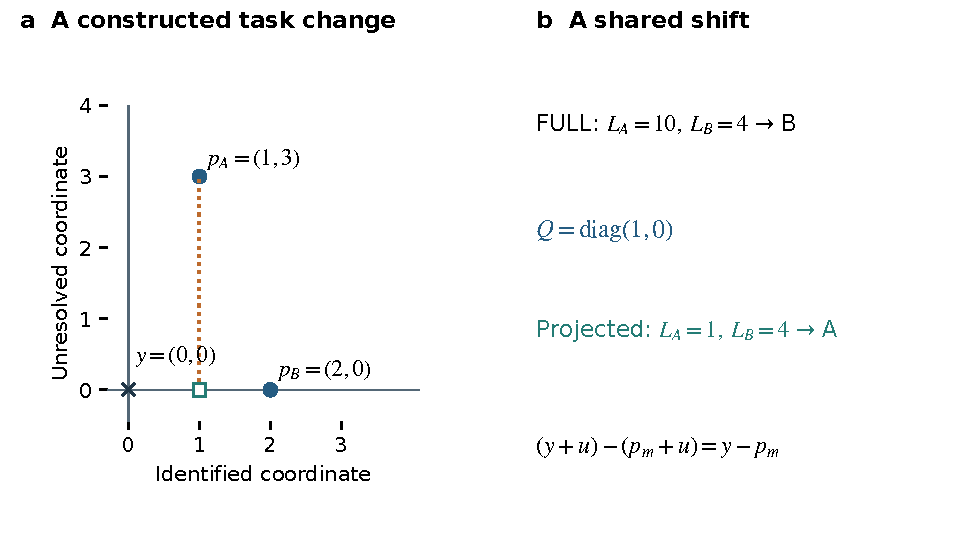
\includegraphics[width=\textwidth]{figures/supp_figure_03.pdf}
\caption{A constructed two-coordinate example distinguishes changing the scored task from a shared reference action. The second coordinate is unresolved. Projecting onto the first coordinate changes the lower-loss model from B to A. A shared translation of truth and predictions changes neither residual, so it cannot change either full squared loss. These numbers are illustrative. Vector diagram prepared with author-reviewed AI-assisted code.}
\label{fig:saction}
\end{figure}


\section{Molecular screens and external source binding}


\subsection{K562, HEK293T and ENCODE measurements}
APA affects transcript 3'-end choice and has context-dependent regulatory functions~\cite{tian2017apa,gruber2019apa,mitschka2022apa}. The K562 APA lineage derives from the published multiplexed single-cell APA regulator screen~\cite{kowalski2024cpa}. The frozen structural panel contains 150 nested inner splits used for legal-space and repair analyses. The strict new-event task groups event identities and biological replicate observations so that an event cannot leak across train and test through duplicate measurement. Five prespecified folds define the aggregate replicate statistic in Supplementary Section~S2.2.2 and use the declared shared non-target-control source ledger.

The independent HEK293T PAS-seq lineage follows Jagannatha et al.~\cite{jagannatha2026rbp}. Its frozen post-QC support contains 30,198 perturbation--event pairs and 1,285 events, with 38 perturbations meeting the replicated-perturbation criterion. The final source ledger uses corrected event-by-batch control identities on the same frozen support and folds. The study is interpreted as a cross-study method-capability recheck rather than an identical-effect replication.

The ENCODE-derived panel uses 235 RBP perturbation experiments, 506,626 skipped-exon events and 10,119,835 measured RBP--event pairs under 20 frozen masks~\cite{vannostrand2020rbp,shen2014rmats}. The structural analysis computes legal-space dimensions without changing response values. The frozen prediction consequence uses pre-bound M1, M2 and M3 score lineages; no estimator is introduced or tuned after estimand-specific outcomes are known.


\subsection{Legal dimensions, replicate structure and K562 requests}
\subsubsection{Composite-only geometry}
Across the 150 frozen K562 inner splits, 9,945 held-out regulator--event instances are individually unsupported under the train-defined two-way reference. The rank increment is 7,310, leaving 2,635 independent composite-only directions. Thus 26.50\% of the unsupported coordinate dimension remains available as legal comparative structure. Across 20 ENCODE masks, 973,298 held-out instances are individually unsupported, the rank increment is 916,903, and 56,395 composite-only directions remain (5.79\%).

\subsubsection{Processed-channel common-structure summary}
For a full-row-rank source-safe legal basis $B$ with $\rank(B)>0$, and $G=(BB^\top)^{-1}$ and completed replicate vectors $z_1,z_2$, the reported basis-invariant summary is
\[
\widehat S=\frac{z_1^\top Gz_2}{d},\qquad d=\rank(B).
\]
All five prespecified K562 strict new-event folds are positive (0.082--0.128; source-safe dimension 2,017--2,505). All five prespecified independent HEK293T PAS-seq folds are positive after corrected event-by-batch source binding (0.026--0.054; source-safe dimension 4,927--5,593). These values summarize aggregate common structure rather than per-direction reproducibility. The two stored processed channels for one assay must not be counted as two independent biological studies; five folds are repeated analysis exposures, not independent experimental replications.

\subsubsection{Relation-query terminals}
The frozen K562 relation panel contains 3,125 queries. Its \emph{archived producer table} records 2,776 \texttt{NOT\_IDENTIFIABLE} and 349 \texttt{COMPARATIVE\_ASSERTABLE} terminals. Historical internal checks report FSPR $=0/2776$, LQR $=349/349$, and CRR $=349/349$; these are archived production-contract metrics rather than newly source-certified output. A subsequent conditional reconstruction from processed \texttt{consensus\_effect} and a TRAIN reference inferred from Q1 identities reproduces the 3,125 saved statuses and all 349 values to maximum absolute error approximately $2.3\times10^{-14}$ using ordinary least squares. Neither status agreement nor arithmetic agreement authenticates the original TRAIN mask, per-query $R_R,R_E$ source action or V1.0.1 producer call lineage. Thus the independent source-certification state remains \texttt{HOLD}; see S10 and S15. These counts are separate from the post-hoc prediction diagnostic in S8.


\begin{figure}[htbp]
\centering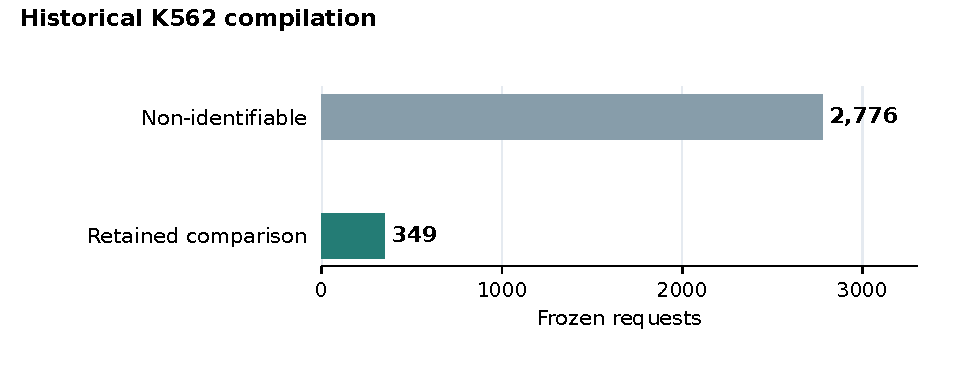
\includegraphics[width=\textwidth]{figures/supp_figure_02.pdf}
\caption{Archived fold-0 K562 producer statuses: 349 recorded comparative terminals and 2,776 nonidentifiable terminals among 3,125 requests. These saved labels and their later conditional numerical replay are not independent authentication of the original source ledger. Plot prepared with author-reviewed AI-assisted code.}
\label{fig:squeries}
\end{figure}


\subsection{Replogle source identities and measurement transformations}
\subsubsection{Source authority}
The external validation required source-native author-released artifacts rather than scPerturb, GEARS, Systema, Hugging Face or other benchmark/re-hosted derivatives. Source recovery established the following primary objects.

\begin{table}[htbp]
\centering
\caption{Key Replogle source-native artifacts used during binding. Full SHA256 identities are listed below the table to preserve readable column widths.}
\small
\begin{tabularx}{\textwidth}{@{}>{\raggedright\arraybackslash}L{0.27\textwidth}>{\raggedright\arraybackslash}L{0.19\textwidth}>{\raggedright\arraybackslash}X@{}}
\toprule
Artifact & Authority & Frozen role \\
\midrule
Raw bulk & Figshare+ DOI 20029387, file 35773070 & Authentic bulk object; rejected for source-aware primary analysis because gem-group identity is absent. \\
KD6 manifest & Figshare+ DOI 20022944, file 35773886 & Library/FASTQ/BAM manifest with gemgroup labels; not used to reconstruct hidden single-cell source identities. \\
Raw single-cell & Figshare+ file 35773219 & Primary V3 source object; 310,385 cells $\times$ 8,563 genes; all four source roles bound. \\
Normalized single-cell & Figshare+ file 35773075 & Source-native secondary sensitivity object; not used as the primary source-safety measurement. \\
\bottomrule
\end{tabularx}
\end{table}

\noindent\textbf{Frozen artifact identities.}\par
\begingroup\small
\setlength{\parindent}{0pt}\setlength{\parskip}{2pt}
Raw bulk SHA256: \texttt{\seqsplit{80de95e54fcbca0e0537d569b43ec92fde6bd0482801505504baebe3118dcadf}}.\par
Raw single-cell SHA256: \texttt{\seqsplit{3e5a63a9e892b21029bb55fca4e12517a49aad7af6c14133ca63d12cf68c6cee}}.\par
Normalized single-cell SHA256: \texttt{\seqsplit{f6967f756b20448641607e1f2a63609681fdf211bf6953971d832e0a32706b73}}.
\endgroup

The raw and normalized single-cell objects have the same byte size (10,661,879,995) but different SHA256 values. Their cell barcodes, perturbation labels, gem-group ordering and response-gene identifiers were matched before outcome opening. The single-cell source roles are: perturbation $\rightarrow$ \texttt{obs.gene\_transcript}; gem group $\rightarrow$ \texttt{obs.gem\_group} (1--48); response feature $\rightarrow$ \texttt{var.gene\_id}; control set $\rightarrow$ 97 source-native non-targeting categories. These 97 categories equal the bulk \texttt{core\_control==True} set.

\subsubsection{Why the normalized V2 contract was superseded}
The author-released normalized expression is defined within gem group and gene using a control-derived mean and standard deviation. If
\[
Z_i=\frac{X_i-\mu_{\rm ctrl}}{\sigma_{\rm ctrl}},
\]
where $\mu_{\rm ctrl}$ is the arithmetic mean of the same control cells and $\sigma_{\rm ctrl}\ne0$, then
\[
\operatorname{mean}(Z_{\rm ctrl})=0
\]
is an algebraic identity. A later construction $Y=P(Z)-C(Z)$ therefore has $C(Z)=0$ by definition while control-derived $\sigma_{\rm ctrl}$ remains embedded in the perturbation values. Representing this dependence as a simple additive \texttt{CTRL::b::g} term with coefficient $-1$ is incorrect. The corresponding V2 terminal was therefore superseded as \texttt{SUPERSEDED\_\_SOURCE\_SEMANTICS\_MISMATCH}. No $Y$, panel, query or scientific result existed under V2.

\subsubsection{Final V3 source-linear measurement}
The primary V3 transformed expression is
\[
\widetilde X_{ig}=10^4 X^{\rm raw}_{ig}/\mathrm{UMI}_i,
\]
using source-native \texttt{obs.UMI\_count}. All 310,385 UMI denominators are finite, positive integers. Control-adjusted UMI counts, control-derived scale factors and gem-group z-scores are explicitly excluded from the primary scale.

For gem group $b$, perturbation $p$ and response gene $g$,
\[
P_{bpg}=\frac{1}{n_{bp}}\sum_{i\in(b,p)}\widetilde X_{ig},\qquad
C_{bg}=\frac{1}{n_{b,\mathrm{NTC}}}\sum_{i\in(b,\mathrm{NTC})}\widetilde X_{ig},
\]
and
\[
Y_{bpg}=P_{bpg}-C_{bg}.
\]
The declared source atom \texttt{CTRL::b::g} is $C_{bg}$ and enters every matching $Y_{bpg}$ with exact coefficient $-1$. The 12 bulk-only names that contain non-targeting text but are not marked \texttt{core\_control} and are absent from the single-cell control set are excluded.


\subsection{Eligibility, outcome-blind panel selection and query families}
\subsubsection{Support layers}
Measurement existence and relation-query eligibility are intentionally different. A measurement row exists for $n_{bp}\ge1$ and $n_{b,\mathrm{NTC}}\ge2$. All 48 gem groups satisfy the control rule with at least 116 NTC cells. A relation query additionally requires at least $K=4$ supported gem groups. The value $K=4$ is metadata-only: it is the largest integer that retains all 2,176 targeting perturbation identities; $K=5$ would remove one. It is not justified as a precision threshold.

All 8,563 unique \texttt{var.gene\_id} values define the candidate response universe. No gene is filtered by mean expression, variance, dropout, CV, Fano factor, differential expression or biological effect. The logical pair identity space is 18,633,088.

\subsubsection{Pre-outcome numeric panel}
All eligible perturbations are retained. Exactly 256 response genes are selected by deterministic identifier-only SHA256 ordering using the canonical key
\begin{center}
\texttt{REPLOGLE\_GENE\_PANEL\_V1::gene\_id}.
\end{center}
No expression value enters panel selection.

\subsubsection{Query families}
The reference model is
\[
Y_{bpg}=\mu+\alpha_p+\beta_g+\delta_b+\Gamma_{pg}+\varepsilon_{bpg}.
\]
No arbitrary sum-to-zero or reference constraint is used to manufacture an atomic estimand. Four relation families are frozen:
\begin{align*}
\mathrm{Q1}:&\quad \Gamma_{pg},\\
\mathrm{Q2}:&\quad \Gamma_{p_1g}-\Gamma_{p_2g},\\
\mathrm{Q3}:&\quad \Gamma_{pg_1}-\Gamma_{pg_2},\\
\mathrm{Q4}:&\quad \Gamma_{p_1g_1}-\Gamma_{p_1g_2}-\Gamma_{p_2g_1}+\Gamma_{p_2g_2}.
\end{align*}
Q2--Q4 candidate queries were canonicalized, SHA256-ranked and frozen before expression access. Common-gem-group support and equal weighting are part of the frozen query definition. Q4 averages the four-term difference over that common support. The response-row coefficients cancel perturbation, gene and batch margins, giving $a^\top X_E=0$ and zero reference-row completion. The external assay contract is not a new prediction train/test split; the adapter's raw measurement coefficients must not be confused with the reference-row $h$ in S1.1.3. Query canonical strings and hashes were sealed before the first access to $X$ values.

\subsubsection{Geometry result}
The four query families have distinct eligibility states, summarized in Table~\ref{tab:externalgeometry}. These states separate reference-identifiability from declared source safety.
\begin{table}[htbp]
\centering
\caption{External geometry and final claim interpretation.}
\label{tab:externalgeometry}
\small
\begin{tabularx}{\textwidth}{@{}L{0.12\textwidth}L{0.16\textwidth}L{0.16\textwidth}X@{}}
\toprule
Family & Identifiable & Source-safe & Interpretation \\
\midrule
Q1 & No & No & Atomic pair effect is not a reference-invariant relation and also retains declared control dependence. \\
Q2 & No & Yes & Shared control cancels, proving source-safety does not imply identifiability. \\
Q3 & No & No & Same-perturbation, cross-gene contrast remains outside both legal sets. \\
Q4 & Yes & Yes & Legal query design under the declared additive control ledger; 100,000 frozen Q4 structures pass the algebraic gates, without new H5AD expression-level effect certification. \\
\bottomrule
\end{tabularx}
\end{table}


\subsection{Why the equal-weight source gate is non-binding}
The statement below concerns the declared additive source design and query identities, not new numerical outputs extracted from the original 10-GB expression matrix. Under V3, each measurement contains $-C_{bg}$. For an equal-weight query over fixed gem-group support, the residual coefficient on source $C_{bg}$ is proportional to the sum of the query coefficients associated with response gene $g$ in gem group $b$. The interaction functionals that are identifiable under the additive nuisance model satisfy the corresponding zero-sum conditions across perturbation and gene margins. Therefore every identifiable equal-weight Q4 functional cancels the declared control source.

The estimability-only comparator C2 and the full source-aware comparator C3 thus accept the same identifiable query set. This equality is mathematical for the frozen V3 design, not an empirical observation that source contamination happened to be absent. The correct terminal field is
\begin{center}
\texttt{\seqsplit{source\_gate\_status = STRUCTURALLY\_NONBINDING\_UNDER\_V3\_EQUAL\_WEIGHT}}.
\end{center}
The historical research archive also records
\begin{center}
\texttt{\seqsplit{demonstrates\_cross\_domain\_quantitative\_compilation = true}},\\
\texttt{demonstrates\_source\_ledger\_increment = false}.
\end{center}


\subsection{Comparator definitions and implementation checks}
Four conceptual comparators distinguish measurement availability from relation support. C0 treats measurement as relation; C1 reports conventional constrained fixed-effect atomic coefficients under alternative reference codings; C2 uses estimability alone; and C3 additionally checks declared-source cancellation.

C1 tests conventional constrained fixed-effect atomic coefficients under alternative reference codings. Its purpose is diagnostic: a coding-dependent atomic coefficient should not be confused with a reference-invariant relation. During independent audit, the intended perturbation-reference-only swap was found to change both perturbation and gene reference. The corrected implementation uses
\begin{center}
\texttt{coding\_b = ref\_atomic(p\_ref\_b, g\_ref\_a)}
\end{center}
so the gene reference remains fixed while the perturbation reference changes. C1 was recomputed from the same frozen $Y$; no panel, query, measurement or outcome-selection rule changed. The corrected diagnostic score is 0.99609375 rather than the superseded 0.999996\ldots value. The audit confirms that atomic coefficients move under coding while legal Q4 contrasts remain invariant.

The final independent audit also added an explicit Q3-independence assertion, terminal-file authority, custody hashes, a self-consistent SHA256 manifest without \texttt{PENDING\_SELF}, nonzero process exit for STOP terminals, and a guard that \texttt{numerically\_resolved=1} is not itself sufficient for a legal quantitative answer. The final audit recorded zero failures.


\subsection{Quantitative recomputation and evidence scope}
The authoritative terminal is stored in \texttt{11\_final/TERMINAL.json}; a PASS clears any stale \texttt{STOP.json}. Custody hashes seal raw input identity, support geometry, alignment and $Y$. The independent audit re-computed 200 deterministic Q4 estimates directly from frozen $Y$ and matched the primary output. The full legal quantitative set contains 100,000 queries, all Q4. No post-outcome rescue dataset, alternative query family, weighting change or source model was introduced.

The supported external result is quantitative compilation under the final source-native contract. Q2 provides a useful logical control because it is source-safe but non-identifiable. The retained Q4 queries reuse perturbations, genes and controls; their number does not count independently validated mechanisms. Source gating introduces no additional rejection among the identifiable equal-weight queries, and measurement existence alone establishes neither precision nor significance.



\section{APA prediction replay and component-specific scoring}


\subsection{Historical K562 predictive anchor}
Across 50 frozen outer test masks, the historical low-dimensional B2 baseline has MSE 0.1129436318 versus 0.1905898683 for zero D3, a reduction of 40.740\% (95\% interval 33.106--46.961\%). The historical baseline reductions are positive in 50/50 outer masks and 31/32 regulators. The CARE candidate has a 0.3304\% point gain over JFE-WALS, with crossed 95\% interval $[-5.2027\%,+5.0266\%]$, and does not meet the frozen stronger-comparator criterion. A lower descriptive point loss therefore does not establish superiority. The original prediction panel, masks and gate remain fixed; the aggregation analysis below asks a different question from predictor superiority.



\subsection{Archived predictions and aggregation contracts}

Read-only replay of the archived PAIR-CARE development package used 387,000 stored prediction rows, 129,000 fold-local pair units, 50 outer folds and three stored solver realizations. The primary mean squared losses reproduce the inherited adjudication to $6.94\times10^{-17}$; original row-loss errors are at most $5.33\times10^{-15}$. The stored identifiers cover 11,917 pair IDs, 32 regulators and 777 event IDs. The later native-mask check shows that this is exactly the union of all declared outer TEST sets within a processed universe of 12,898 pairs and 1,140 events; 981 pairs and 363 events never enter those TEST sets. This does not rebind a raw exact-PAS atlas.

The same stored predictions demonstrate the classical identity
\[
\frac1S\sum_s(y-p_s)^2=(y-\bar p)^2+\frac1S\sum_s(p_s-\bar p)^2.
\]
For CARE versus JFE-WALS, the stored-realization mean-loss difference is $-0.0003639155$, whereas scoring the mean predictions gives $+0.0005927712$. A streaming checker independently reproduces both. One of all 15 comparisons in the fixed six-model panel changes point order. This is a difference between prediction/aggregation contracts; it is not a confidence-supported winner, a reference-completion ambiguity or a successful CARE upgrade. The original CARE gate remains STOP.

The original archived-prediction subset alone did not contain reference masks. The subsequently recovered native processed response and masks now support the direct support and reference-target reconstructions in S6.2.3. Completed raw measurement/source operators and biological-arm covariance remain unavailable. The extended replay therefore certifies processed-input consistency, not source-native measurement precision or a minimum-cost physical assay design.





\begin{figure}[htbp]
\centering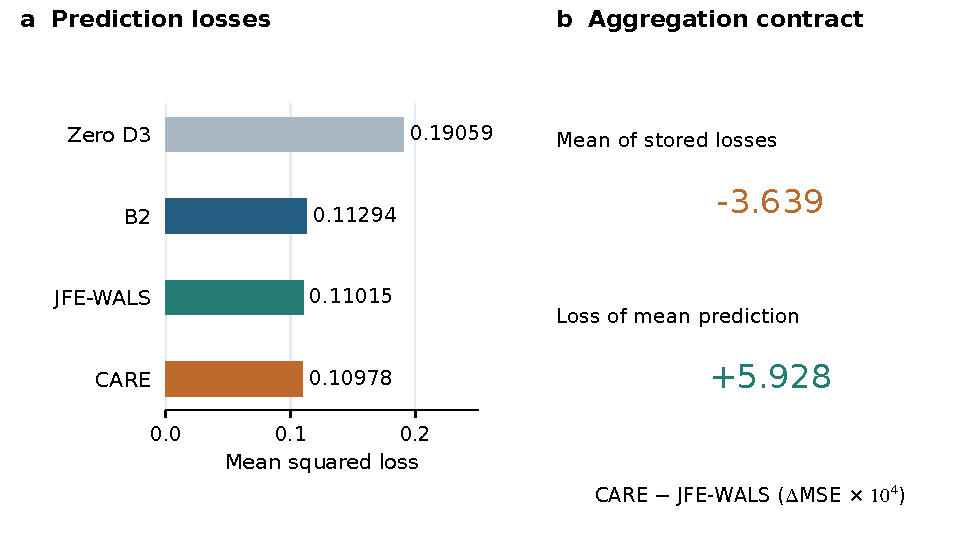
\includegraphics[width=\textwidth]{figures/supp_figure_01.pdf}
\caption{Archived APA prediction losses and the aggregation-dependent CARE--JFE-WALS point order. The left panel replays fixed prediction losses; the right compares mean stored-realization loss with loss of the mean prediction. Displayed values are descriptive, without a new uncertainty interval. This change of aggregation leaves the failed CARE upgrade unchanged. Vector diagram prepared with author-reviewed AI-assisted code.}
\label{fig:saggregation}
\end{figure}


\subsection{ENCODE estimand-dependent ordering}
The frozen ENCODE comparison uses the same stored M1 additive, M2 SVD-50 and M3 additive-plus-LR-25 predictions on two legal components. Composite-only loss is 0.004313275, 0.002321316 and 0.003172774 for M1, M2 and M3, respectively; unitwise-supported loss is 0.005812259, 0.004293260 and 0.004060695. Their descriptive orders differ: M2 $<$ M3 $<$ M1 on composite-only components and M3 $<$ M2 $<$ M1 on unitwise support. The values are the frozen plotting inputs and are not a newly tuned estimator comparison.



\begin{figure}[htbp]
\centering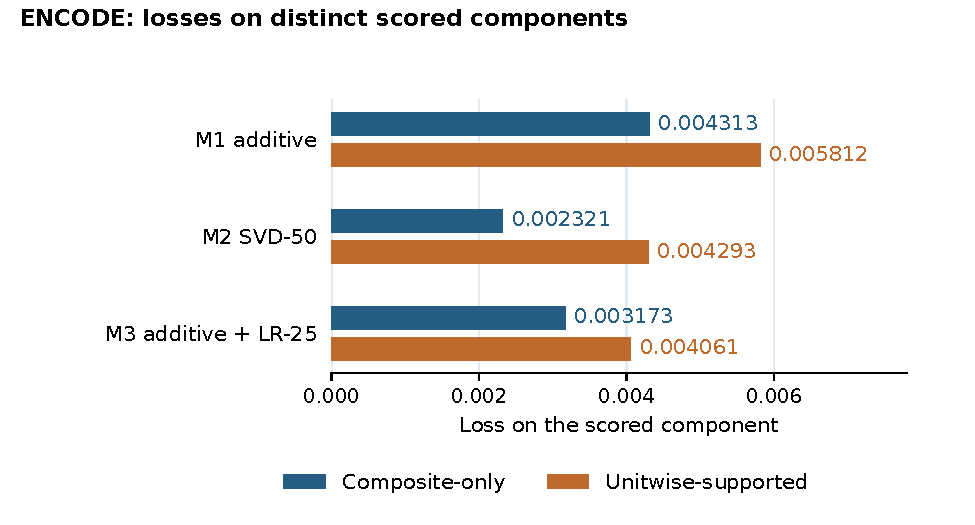
\includegraphics[width=\textwidth]{figures/supp_figure_04.pdf}
\caption{The same ENCODE predictions evaluated on different legal components. The component-specific orders differ without changing predictions. Values have their original loss definitions; neither order invalidates the other target. Plot prepared with author-reviewed AI-assisted code.}
\label{fig:sencode}
\end{figure}


\section{Drug-response evaluation and confirmation analyses}


\subsection{Design-only evaluation geometry}
The Stage-0 authority was DrEval v1.4.1 with CTRPv2. After the paper-era missing-measure filter, the bound universe contained 235,974 rows, 231,628 distinct cell--drug pairs and 886 cell lines. All training graphs were connected. Across ten folds:
\begin{itemize}
\item LPO: $\rank(U)=0$ in every fold; five primary metrics were target-evidence-identifiable.
\item LCO: $\rank(U)=88$ or $89$, exactly matching the held-out-cell indicator span.
\item LDO: $\rank(U)=54$ or $55$, exactly matching the held-out-drug indicator span.
\item The LCO/LDO quotient equaled within-held-out-entity centering under the ordinary connected topology.
\item MSE was classified as target-completion-dependent but score-invariant; pooled Pearson, $R^2$, normalized Pearson and normalized $R^2$ were score-completion-dependent.
\end{itemize}
No prediction or outcome value was opened to obtain these structural classifications.


\subsection{CTRPv2 fixed-prediction consequence}
The official Springer Nature Figshare DrEval Source Data artifact was bound as article 30724907, file 63690570, size 5,580,538,652 bytes, SHA256
\begin{center}\small
\texttt{\seqsplit{676f5d7eb5a0615edf21fbe24719e5e8f3783efeeac35d916dab447a87cba060}}.
\end{center}
Published scores were reproduced before quotient scoring. LPO remained the identity control. LCO was stable on the integrity-valid three-model panel ($\tilde\tau=1$, median reversal $0$). LDO used seven non-naive models and produced:
\begin{center}
\begin{tabular}{@{}lccc@{}}
\toprule
Metric & Median $\tau$ & Median reversal & Persistent pairs \\
\midrule
normalized $R^2$ & 0.000 & 0.500 & 3 \\
normalized Pearson & 0.286 & 0.357 & 2 \\
\bottomrule
\end{tabular}
\end{center}
The five persistent model-pair--metric results (four distinct model pairs) were:
\begin{itemize}
\item ElasticNet--RandomForest (nR2, 7/10);
\item MultiOmicsNeuralNetwork--MultiOmicsRandomForest (nR2, 7/10);
\item MultiOmicsNeuralNetwork--RandomForest (nR2, 8/10);
\item MultiOmicsNeuralNetwork--RandomForest (nPearson, 7/10);
\item RandomForest--SimpleNeuralNetwork (nPearson, 7/10).
\end{itemize}
The top model ranked by the arithmetic mean normalized $R^2$ over ten LDO folds changed from MultiOmicsNeuralNetwork (0.02346627875) to DIPK (0.02118309114). The fold-wise modal winner is a separate aggregation. These are fixed-prediction evaluation consequences, not claims that DIPK is universally superior.


\subsection{GDSC primary and secondary confirmation}
Stage 2 prospectively fixed GDSC2 as primary and GDSC1 as secondary. The CLI response token \texttt{LN\_IC50} resolves under the paper-era loader to \texttt{LN\_IC50\_curvecurator}. Correct final universes were 90,666 rows/287 drugs (GDSC2) and 158,808 rows/378 drugs (GDSC1).

Seven Stage-1 candidate models entered outcome-independent feature/support audit. The primary common-support rule selected six models that preserve the complete base held-out-drug universe in all ten folds: ElasticNet, GradientBoosting, RandomForest, SimpleNeuralNetwork, MultiOmicsRandomForest and MultiOmicsNeuralNetwork. DIPK remained executable on model-specific support but was secondary-only because missing MolGNet support removed held-out drugs. Primary evaluation support was the fold-wise common row intersection across the six models; mean support was 8,274.9 rows/fold for GDSC2 and 14,560.8 rows/fold for GDSC1. All held-out drugs were preserved and each retained at least two rows.

Nine of ten folds in each resource had the ordinary within-held-out-drug quotient topology. The exceptions are different: GDSC2 fold 6 has a nested rank mismatch, whereas GDSC1 fold 5 has a tilted equal-rank space relative to ordinary centering (S4.7). Both use their frozen general operator; equal rank does not prove equal subspace. The models were trained and tuned under the frozen DrEval v1.4.1 procedure; PAIR information was not used for tuning. One naive baseline was sealed per fold and shared across all six models. Each resource sealed 60 primary model-fold prediction artifacts and ten naive folds before scoring.

\begin{center}
\small
\begin{tabular}{@{}lcccccc@{}}
\toprule
Resource & nR2 $\tilde\tau$ & nR2 rev. & nPearson $\tilde\tau$ & nPearson rev. & Persistent & Top change \\
\midrule
GDSC2 & 0.40 & 0.30 & 0.40 & 0.30 & 0 & 7/10 \\
GDSC1 & 0.27 & 0.37 & 0.33 & 0.33 & 0 & 7/10 \\
\bottomrule
\end{tabular}
\end{center}
The frozen Level-B criterion required, within the same metric, median reversal $\ge0.10$ and at least one pair reversing in the same direction in $\ge7/10$ folds. The first component passed in both resources, but persistence failed. ElasticNet--RandomForest under normalized $R^2$ was the nearest carrier at 6/10 in both resources. Accordingly, GDSC2 entered the frozen primary STOP state (structure replicated but the persistent decision-effect criterion did not), GDSC1 entered the frozen secondary structure-only STOP state, and the Stage-2 program terminal remained the prespecified primary-confirmatory-replication failure recorded in S6.5.


\subsection{Metric ties and the prespecified persistence criterion}
For each fold and primary metric, model rankings under the published and quotient contracts were compared using Kendall's $\tau$, all ordered model-pair directions, reversal fraction, top-model identity and top-three overlap. Numerical ties used the frozen tolerance
\[
\max\{10^{-12},100\epsilon\max(1,|s_i|,|s_j|)\},
\]
and tie-to-ordered transitions were not counted as reversals. A persistent reversal required the same ordered pair to change in the same published-to-PAIR direction in at least 7/10 folds. The prespecified Stage-2 Level-B replication gate required, within the same metric, median foldwise reversal fraction $\ge0.10$ and at least one persistent non-naive pair. The primary GDSC2 terminal was fixed by this gate; GDSC1 could not rescue a failed primary adjudication. Level C was descriptive only and was not used to determine the program terminal.


\subsection{Fingerprint-only support sensitivity}
The four fingerprint models share larger row support than the MultiOmics models. Without retraining or HPO, the secondary analysis rebuilt $Q$ on the enlarged fingerprint-only common support. GDSC2 gained a mean 565 rows/fold and GDSC1 gained 997. Median reversal was 0.33/0.33 (nR2/nPearson) in GDSC2 and 0.42/0.33 in GDSC1, persistent pairs remained zero, and ElasticNet--RandomForest nR2 remained 6/10. The larger support does not recover persistence in this sensitivity analysis; it does not rule out all effects of support composition or resource heterogeneity. The optional DIPK reduced-drug-universe secondary was not executed.


\subsection{Squared-error decomposition and common support}
For squared-error comparison of two frozen predictions $p_A,p_B$ on one shared support, let $Q$ be the evidence-identified projector and $P=I-Q$. Orthogonality gives
\[
\Delta_{\mathrm{FULL}}
=
\left[\|Q(y-p_A)\|_2^2-\|Q(y-p_B)\|_2^2\right]
+
\left[\|P(y-p_A)\|_2^2-\|P(y-p_B)\|_2^2\right]
=
\Delta_{\mathrm{ID}}+\Delta_{\mathrm{UNRES}}.
\]
This equality uses the unweighted Euclidean geometry on the expanded observation multiset (or a common scalar normalization). A general diagonal weighting would require a matching weighted-orthogonal projector; Euclidean orthogonality alone is not sufficient. Under the frozen scoring weights, the identity is exact and provides a mechanism for FULL--PAIR rank changes. It is not extended to Pearson correlation.

The historical WP4 common-support audit separately tests the model-specific-scoreability explanation within its certified supports. Historical normalized-$R^2$ contained 102 strict FULL--PAIR reversals under the audited support semantics. Of these, 55 admitted native exact certificates and 47 were certified after pairwise common-support transport. All five historical pair--metric persistence results remained persistent and the top-model change MultiOmicsNeuralNetwork $\rightarrow$ DIPK was preserved. The audit therefore closed with the historical decision consequence intact rather than by reducing eligible folds or silently dropping unsupported rows.


\subsection{General projection versus centering}
The general quotient was compared fold-by-fold with the simple within-held-out-drug centering operator.
\begin{center}
\small
\begin{tabular}{@{}lll@{}}
\toprule
Fold class & Structural result & Frozen ranking consequence \\
\midrule
18/20 GDSC folds & Equivalent within tolerance & Identical by construction \\
GDSC1 fold 5 & Tilted, equal rank; $\sin\theta\approx0.0126641$ & No disagreement \\
GDSC2 fold 6 & Centering subspace strictly nested in general space & No disagreement \\
\bottomrule
\end{tabular}
\end{center}
For GDSC1 fold 5, the single-angle equal-rank projector distance is $\sqrt{2}\sin\theta\approx0.0179097$. Across the frozen GDSC model comparisons, general $Q$ versus centering produced 0/300 ranking disagreements for normalized $R^2$ and normalized Pearson. The correct interpretation is structural generality without a frozen empirical ranking increment.

The independent certificate audit also corrected an implementation issue in an earlier non-equivalence witness: a left singular vector could lie outside the intended keep subspace. The final certificate maps right-singular coefficients back to the original space and explicitly verifies membership before adjudication. This correction changed implementation certification, not the frozen ranking results.


\subsection{A new symmetric-HPO training realization}
The historical prediction cells could not be reconstructed under the original training environment, so the initial exact historical-cell reconstruction stopped because the complete original model panel was not reconstructible. A bounded recovery control then trained a symmetric-HPO panel under the archived DrEval training/prediction path. This wave was explicitly a post-closure reproducibility stress test, not a rescue of the frozen Stage-2 program.

All 560 authorized R0 jobs completed. Final prediction and HPO lineage checks, model/fold row counts and independent score recomputation passed the final 31/31 integrity closeout. During audit, a scorer helper was found to collapse duplicate $(\mathrm{cell},\mathrm{drug})$ keys, whereas the historical WP4 evaluator uses pandas left-join semantics that can expand duplicates Cartesianly. The live scorer was changed to the single historical merge semantics without retraining and retained fail-closed checks for missing NaiveMeanEffects rows, truth mismatch and support consistency. Historical published predictions replayed through this same final scorer recovered the frozen counts exactly:
\[
7/10,\quad 7/10,\quad 8/10,\quad 7/10,\quad 7/10.
\]
The symmetric-HPO predictions produced:
\[
5/10,\quad 6/10,\quad 7/10,\quad 6/10,\quad 5/10,
\]
in the same pair/metric order. Only MultiOmicsNeuralNetwork--RandomForest under normalized $R^2$ met the unchanged 7/10 threshold. The terminal is therefore
\begin{center}
\texttt{STOP\_\_WP5B\_R\_R0\_\_CONTROL\_REPRODUCTION\_INSUFFICIENT}.
\end{center}
The planned GroupMean and subsequent training branches were not executed.

This result leaves two statements simultaneously true. First, the historical Stage-1 decision consequence exists and is reproducible from its frozen prediction artifact; the final scorer is capable of recovering it exactly. Second, the five specific historical pair--metric results are not established as stable outputs of the newly instantiated learning procedure. Because only one new realization was produced and multiple training/software-history factors differ from the unreconstructible historical cells, the R0 contrast is not interpreted as a causal HPO effect or as an estimate of $P(\Delta>0)$ under future retraining.


\section{Conditional decision and information certificates}


\subsection{Quadratic loss-difference ranges}
All weights, row identities, multiplicities, finite masks and action maps are fixed within a certificate. For $y(t)=y+T_yt$ and $p_m(t)=p_m+T_mt$, let $D_m=T_y-T_m$ and $e_m=y-p_m$. Expanding the two original weighted squared losses gives
\[
\Delta(t)=c+2\ell^\top t+t^\top Ht,
\]
with $c=e_A^\top We_A-e_B^\top We_B$, $\ell=D_A^\top We_A-D_B^\top We_B$ and $H=D_A^\top WD_A-D_B^\top WD_B$. Here $H$ is symmetric and $W\succeq0$. The shared-action case has $D_A=D_B=0$; the truth-only case has $D_A=D_B=T_y$ and therefore $H=0$.

\begin{proposition}[Constancy, finite bounds and exact sign decisions]
The polynomial is constant over $\R^r$ iff $H=0$, $\ell=0$. If $H\succeq0$ and $\ell\in\operatorname{col}(H)$, its minimum is $c-\ell^\top H^+\ell$, attained at $t=-H^+\ell+v$ for $v\in\ker(H)$. Otherwise its infimum is $-\infty$. Applying this to $-\Delta$ determines the supremum. Every intermediate value between the infimum and supremum is attained, with finite endpoints attained.
\end{proposition}
\begin{proof}
Constancy forces the linear and quadratic coefficients to vanish, for example by evaluating along each coordinate direction and their sums. If a vector $v$ satisfies $v^\top Hv<0$, the quadratic term makes $\Delta(sv)\to-\infty$ as $|s|\to\infty$. If $H\succeq0$ but $\ell\notin\operatorname{col}(H)$, the orthogonal projection of $\ell$ onto $\ker(H)$ is nonzero and a signed multiple of it gives an unbounded linear decrease. Otherwise completing the square gives
\[
\Delta(t)=(t+H^+\ell)^\top H(t+H^+\ell)+c-\ell^\top H^+\ell.
\]
The maximum follows by sign reversal. Continuity and connectedness of $\R^r$ imply an interval of attained values; the displayed optimizers attain finite endpoints.
\end{proof}
The resulting statuses are: invariant loss difference; variable loss difference with a strictly invariant winner; two attainable strict orders; one-sided order with a tie boundary; and numerically unresolved. Score non-invariance alone does not select among these decision states. A value bound is not a confidence interval. Restricting the completion space to a biologically motivated bounded region requires a new declared region and a different optimization certificate, not silent truncation of this result.

Negative-curvature or null-linear directions construct unbounded witnesses. Finite endpoints provide minimizers/maximizers. The implementation searches a finite scale along a certified unbounded direction only to serialize an explicit sign witness, then independently evaluates both original weighted losses there. A numerical witness cannot certify a global relation merely by testing many sampled completions.

For fixed predictions and a truth-only action $y(t)=y+Ut$, the quadratic terms cancel and the exact difference reduces to
\[
\Delta_{A,B}(t)=\Delta_{A,B}(0)+2t^\top U^\top W(p_B-p_A).
\]
If its slope is nonzero, both strict orders are attainable over $t\in\mathbb R^r$; if the slope is exactly zero, the difference is constant. The magnitude of a nonzero slope does not change this unbounded-domain conclusion. Treating a small coefficient as zero therefore requires a different, explicitly bounded domain or an unresolved numerical status. Under the shared action on truth and both predictions, every residual is unchanged instead, as shown in S1.6.

For normalized $R^2$, the quadratic certificate may be used to decide its order only when a common positive denominator and common support justify the SSE reduction. No such reduction is assumed for Pearson, median aggregation across different supports, clipping, or an opaque evaluator primitive.


\subsection{Prospective exact linear information}
Suppose the goal is to determine the full polynomial $\Delta(t)$ from exact additional linear information $Kt$ for every possible information value. This is stronger than certifying a single winner and different from constancy on one particular observed fiber.

\begin{proposition}[Necessary and sufficient calibration factorization]
There is a function $f$ with $\Delta(t)=f(Kt)$ for all $t$ iff
\[
\ker(K)\subseteq\ker(H)\cap\ker(\ell^\top).
\]
The minimum dimension of arbitrary exact linear information is $\rank([H;\ell^\top])$.
\end{proposition}
\begin{proof}
For $v\in\ker(K)$, factorization requires $\Delta(t+v)-\Delta(t)=0$ for every $t$. This difference equals $2t^\top Hv+v^\top Hv+2\ell^\top v$. Its vanishing for all $t$ requires $Hv=0$ and then $\ell^\top v=0$. These conditions are also sufficient. By row/null-space duality, the row space of $K$ must contain that of $[H;\ell^\top]$. A row-space basis attains the rank lower bound.
\end{proof}
For a finite family $\Delta_j=c_j+2\ell_j^\top t+t^\top H_jt$, stack all $H_j$ and $\ell_j^\top$ to obtain the corresponding minimum dimension. A basis of this stacked row space is a constructive information certificate.

\Needspace{20\baselineskip}
\subsubsection{Exact decision information when ties remain distinct}
Let $d(t)=\operatorname{sgn}\Delta(t)\in\{-1,0,+1\}$ distinguish an A win, a tie and a B win. The domain is all of $\mathbb R^r$, and additional information is exact and linear. These choices matter: a binary tie-breaking rule, a bounded domain, approximate decisions and noisy measurements are different problems.

\begin{proposition}[Decision information dichotomy for a quadratic]
\label{prop:decisioninformation}
If $d$ is constant, no additional information is required. Otherwise, there exists a function $g$ such that $d(t)=g(Kt)$ for every $t\in\mathbb R^r$ if and only if
\[
\ker(K)\subseteq\ker(H)\cap\ker(\ell^\top).
\]
Consequently the minimum number of arbitrary exact linear coordinates is
\[
r_{\rm decision}=\begin{cases}
0,&d\ \text{is constant},\\
\operatorname{rank}\!\begin{bmatrix}H\\\ell^\top\end{bmatrix},&d\ \text{is nonconstant}.
\end{cases}
\]
\end{proposition}
\begin{proof}
Sufficiency follows from factorization of the full polynomial. For necessity let $v\in\ker(K)$; every line $t+sv$ must have a constant decision. If $\Delta$ takes both positive and negative values, $v^\top Hv>0$ would change the sign along a line through a negative point for large $|s|$, while $v^\top Hv<0$ would do so through a positive point. Hence $v^\top Hv=0$. The restriction to every such line is now affine, with slope $2(t^\top Hv+\ell^\top v)$. A nonzero slope attains both signs, so the slope must vanish for every $t$, giving $Hv=0$ and $\ell^\top v=0$.

The remaining nonconstant case is a polynomial of one weak sign that attains zero. Suppose $\Delta\ge0$ and $\Delta(t_*)=0$. Then $H\succeq0$, $Ht_*+\ell=0$ and $\Delta(t)=(t-t_*)^\top H(t-t_*)$. Preservation of the tie along $t_*+sv$ requires $v^\top Hv=0$, which for positive-semidefinite $H$ implies $Hv=0$ and then $\ell^\top v=0$. Apply the same argument to $-\Delta$ in the nonpositive case. Row/null-space duality gives the rank lower bound, attained by a row-space basis of $[H;\ell^\top]$.
\end{proof}
The distinction is operational. For $\Delta=1+t_1^2+t_2^2$, the winner is fixed and $r_{\rm decision}=0$ although $r_{\rm cal}=2$. For $\Delta=t_1^2$, preserving the tie requires one coordinate even though A never wins. For $\Delta=t_1t_2$, two are necessary globally. After exact information has restricted the feasible set to a nonempty affine fiber $t=t_0+Zs$, apply the proposition to $\widetilde H=Z^\top HZ$, $\widetilde\ell=Z^\top(Ht_0+\ell)$ and $\widetilde c=\Delta(t_0)$. This determines the minimum \emph{additional} linear information in the fiber coordinates. For example, observing $t_1=0$ in the last case already certifies a tie; observing $t_1=1$ leaves the sign of $t_2$ unresolved.

The all-space assumption cannot be dropped. On $[-1,1]^2$, the quadratic $t_1(2+t_2)$ has the sign of $t_1$, although its value depends on both coordinates. On $\mathbb R^2$ both coordinates are needed. Likewise, the higher-degree polynomial $t_1(1+t_2^2)$ has globally the sign of $t_1$ without being a function of $t_1$ alone. This is a restricted quadratic completeness result, not a claim of a new general dimension-reduction theory, physical assay savings or predictive improvement.

\Needspace{15\baselineskip}
\begin{proposition}[Fixed-prediction panel bound]
If $y(t)=y+Ut$ and $M$ predictions remain fixed, squared-loss differences are affine. The information needed for all pairwise differences has dimension
\[
\rank\!\begin{bmatrix}(p_2-p_1)^\top WU\\\vdots\\(p_M-p_1)^\top WU\end{bmatrix}\le\min\{r,M-1\}.
\]
If all predictions share the truth action instead, the dimension is zero.
\end{proposition}
\begin{proof}
Quadratic terms cancel under a truth-only action. Every pairwise linear coefficient is the difference of two model coefficients, so coefficients relative to one anchor model span all of them. Under a shared action every residual action is zero.
\end{proof}
For one \emph{observed} calibration value with fiber $t=t_0+Zv$, constancy instead requires $Z^\top HZ=0$ and $Z^\top(Ht_0+\ell)=0$. These conditions can be weaker; they cannot be substituted for the prospective all-values requirement. For example, $\Delta=t_1t_2$ vanishes along the fiber $t_1=0$, but measuring only $t_1$ does not determine it when the observed value is nonzero.

The decision result retains these exact, all-values semantics; a constant winner or an already decisive observed fiber can require less information. The rank is a count of independent exact linear functionals. Restricting calibration to a finite pool of physical measurement rows turns containment into a different constrained selection problem; this supplement does not assert optimal assay count or cost. No noisy-assay guarantee or new biological replication follows from a low rank.


\subsection{Completed measurements, source-aware information and precision}
\label{sec:claiminformation}
This section links the biological, algebraic and decision objects under one declared contract. The individual estimability, minimum-variance and optimal-design results are classical; the candidate contribution is their executable composition with PAIR's reference, source and prediction semantics. They are not presented as first discoveries of the underlying mathematics.

\subsubsection{Biological interpretation and a fixed completed operator}
For regulator $r$ and APA event $e$, the working decomposition is
\[
Y_{re}=\mu+\alpha_r+\beta_e+\Gamma_{re}+\varepsilon_{re}.
\]
Pair specificity concerns variation beyond both marginal axes. For example,
\[
\Psi=Y_{r_1e_1}-Y_{r_1e_2}-Y_{r_2e_1}+Y_{r_2e_2}
=\Gamma_{r_1e_1}-\Gamma_{r_1e_2}-\Gamma_{r_2e_1}+\Gamma_{r_2e_2}+\varepsilon_\Psi.
\]
This is a comparative perturbation response, not proof of direct RNA binding or of a unique molecular mechanism. Missing combinations remain unknown. Unequal source use, nonlinear preprocessing or an undeclared control can prevent the intended cancellation.

Let $N_R$ span $\ker(X_R)$. A query row family $B$ is reference-identifiable exactly when $BX_EN_R=0$. For a fixed declared reference rule $F_R$, its completed readout is
\[
v=Lx_{\rm raw},\qquad L=[-BX_EF_R,\ B],\qquad x_{\rm raw}=(y_R^\top,y_E^\top)^\top.
\]
Here the subscript `raw' denotes the input coordinates of this declared readout, which stack reference and requested measurements; it does not itself establish binding to original sequencing counts. The rule $F_R$ and the population are part of the estimand. Optimizing $F_R$ after seeing outcomes generally changes the readout; it is not automatically a variance improvement for the same biological quantity. If a declared raw-source perturbation is $x_{\rm raw}\mapsto x_{\rm raw}+R_{\rm raw}s$, source cancellation requires $LR_{\rm raw}=0$, where $R_{\rm raw}=[R_R^\top,R_E^\top]^\top$. This raw-coordinate map is distinct from the completed map $J$ of S1.1.4.

\subsubsection{A model comparison is a lower-dimensional measurement claim}
For fixed predictions $p_A,p_B$ in the same readout coordinates and common diagonal weights $W=\operatorname{diag}(w_i)$ with $w_i\geq0$, define $\Delta=L_A-L_B$. Then
\begin{align}
\Delta(x_{\rm raw})&=(Lx_{\rm raw}-p_A)^\top W(Lx_{\rm raw}-p_A)-(Lx_{\rm raw}-p_B)^\top W(Lx_{\rm raw}-p_B)\\
&=\kappa+q^\top x_{\rm raw},\qquad
q=2L^\top W(p_B-p_A),\quad
\kappa=p_A^\top Wp_A-p_B^\top Wp_B.
\label{eq:rawlossclaim}
\end{align}
Thus only the measured direction $q$ affects this fixed-prediction loss difference. A noisy direction orthogonal to $q$ may impair individual response estimates without impairing this comparison. The cancellation of the common squared-truth term is elementary algebra and has precedent in paired risk comparisons. This statement does not allow predictions, support, weights or the reference rule to change silently.

Under the separate truth-only completion action $v\mapsto v+Ut$, the difference is constant exactly when $(p_B-p_A)^\top WU=0$. Under a shared action on truth and both predictions, the residuals are instead unchanged. When prediction actions differ, use the joint-action definition in S1.6 and the quadratic certificate in S5.1; Eq.~\ref{eq:rawlossclaim} is not a substitute for that contract.

If the declared raw measurement vector used for evaluation satisfies $x_{\rm raw}=x_*+\epsilon$, with $E[\epsilon]=0$ and raw-coordinate covariance $\Sigma_{\rm raw}$, and the prediction vectors are conditionally fixed independently of this measurement error, then $\Delta(x_{\rm raw})$ is unbiased for $\Delta(x_*)$ and its variance is $q^\top\Sigma_{\rm raw} q$. Equivalently the readout covariance is $L\Sigma_{\rm raw} L^\top$. This statistical interpretation requires the stated conditional mean and independence assumptions and a covariance bound to the same raw coordinates; it does not follow from numerical estimability alone. Reference observations used to train predictions require explicit conditioning or a joint dependence analysis, not an automatic independence assertion. A source ledger, two biological arms, many solver seeds, or many overlapping folds do not establish these assumptions.

\subsubsection{Sharp deterministic sensitivity, with no automatic confidence meaning}
Suppose the scientific contract supplies a deterministic perturbation set
\[
\mathcal D=\{\delta=\rho S^{1/2}u:\|u\|_2\leq1\},\qquad S\succeq0,\quad\rho\ge0.
\]
By Cauchy--Schwarz, the sharp interval for Eq.~\ref{eq:rawlossclaim} is
\[
[\Delta(x_{\rm raw})-\rho\sqrt{q^\top Sq},\ \Delta(x_{\rm raw})+\rho\sqrt{q^\top Sq}].
\]
If $q^\top Sq>0$, endpoints are attained by $\delta_\pm=\pm\rho Sq/\sqrt{q^\top Sq}$; otherwise the difference is constant on the set. A strict winner is robust on this set only when the interval is strictly on one side of zero. This is a deterministic theorem. Taking $S$ to be a covariance does not make the interval a 95\% confidence interval without a justified coverage radius and sampling model. A radius measured in D3-output coordinates is not automatically realizable by source-native RNA measurements.

\subsubsection{Source-aware calibration and available assay channels}
Write an admissible calibration model as
\[
w=A\theta+J_{\rm cal}s+\eta=\widetilde A\widetilde\theta+\eta,
\qquad\widetilde A=[A,J_{\rm cal}],\quad\widetilde\theta=(\theta^\top,s^\top)^\top.
\]
Here $J_{\rm cal}$ maps the declared sources into calibration channels. The unknown offsets $s$ are included as parameters, rather than assumed absent. A desired biological or linear decision family has rows $C$ and augmented target $\widetilde C=[C,0]$. It is identified exactly when
\[
\ker(\widetilde A)\subseteq\ker(\widetilde C).
\label{eq:sourceclaiminformation}
\]
For sufficiency, row-space inclusion gives a lift $H$ satisfying $H\widetilde A=\widetilde C$, so $Hw$ determines the target in the noiseless model. For necessity, a vector $v$ with $\widetilde Av=0$ but $\widetilde Cv\ne0$ gives two observationally identical parameter states with distinct requested claims. The implementation returns the lift or this ambiguity witness.

If $\Sigma\succ0$ is supplied and $E[w]=\widetilde A\widetilde\theta$, the classical best linear unbiased lift is
\[
H_*=\widetilde C(\widetilde A^\top\Sigma^{-1}\widetilde A)^+
\widetilde A^\top\Sigma^{-1},\qquad
V_*=H_*\Sigma H_*^\top.
\]
For any other unbiased $H=H_*+D$ with $D\widetilde A=0$, the cross terms vanish and
$H\Sigma H^\top=V_*+D\Sigma D^\top\succeq V_*$. This proves the conditional minimum-variance claim, not the adequacy of a biological covariance estimate. A second checker solves the constrained variance problem through a KKT system without using this formula.

The minimum dimension of arbitrary noiseless linear information is not the number of available experiments. If only candidate rows $\widetilde A_i$ with fixed nonnegative costs $c_i$ are physically admissible, a finite design solves
\[
\min_{S\subseteq\mathcal I}\sum_{i\in S}c_i
\quad\text{subject to}\quad
\operatorname{row}(\widetilde C)\subseteq\operatorname{row}(\widetilde A_S),
\quad \operatorname{diag}(V_S)\leq b\ \text{when precision is declared}.
\]
The supplied precision caps $b$ cannot be chosen to rescue observed outcomes. The prototype exhaustively enumerates at most 18 candidate channels and certifies the finite optimum. It makes no scalability claim; larger candidate pools return \texttt{NOT\_EXECUTED}. This is a bounded discrete application of classical experimental-design theory, not a new SOCP algorithm.

\subsubsection{Counterexamples defining the boundaries}
One abstract coordinate $\theta_1+\theta_2$ has information rank one, but two available channels measuring $\theta_1$ and $\theta_2$ separately are both needed. One coordinate measured with independent variance four requires four such observations to reach variance at most one. In a perturbation/control pair, rows $(1,1)$ and $(0,1)$ identify $(1,0)$ through weights $(1,-1)$; the perturbation row alone confounds the effect with an unknown shared source. A declared shared covariance term cancels in the difference, but declaring covariance cannot repair that unknown-mean confounding.

These boundaries are tested in eight named mathematical fixtures, 60 integer-design contracts, six invalid-input cases and one computation-budget case (75 total). Exact rational rank calculations and a separate KKT calculation check the numerical outputs. They are not 75 biological experiments.




\section{Reproducibility and verification coverage}
\noindent\textbf{Archive-scope note.} This section describes older, separately archived author-side reproduction packages. Their directory names and commands identify past execution environments; they are not a promise that every referenced script or original input appears in the standalone \emph{Information Sciences} manuscript ZIP. A separate author-only provenance bundle preserves the historic research archive. Full independently runnable public deposition remains a submission gate.



\subsection{Constructed verification and interpretation}
The author-side extension includes a restricted quadratic-loss compiler, a separate checker that does not call the generator, and a deterministic verification driver. The six rational fixtures cover common reference action, truth-only action, a changing loss difference with one strict winner, a tie boundary, indefinite curvature and a linear term in the null space of a singular positive-semidefinite matrix. Each fixture has independent original-loss witness replay and exact rational coefficient and repair-rank checks. A further 100 random affine contracts check loss reconstruction, row permutation and repeated-observation multiplicity. Shared-reference $R^2$, common-baseline, maximal-invariant, discarded-invariant-information, minimal-information, small-nonzero-term and invalid-domain controls bring the total to 115 checks, all passing.

The random seed is 20261010 and is a software-fixture seed, not a predictive-model seed. Numerical range certificates carry their tolerance and refuse small nonzero curvature or null-linear terms rather than converting them to exact zeros on an unbounded orbit. Structural shared-action cancellation is flagged separately. Numerical row-space ranks remain tolerance-dependent unless checked exactly, as done for the six rational fixtures.

\begin{table}[htbp]
\centering\small
\caption{Constructed verification cases. These are proof/software fixtures, not biomedical validation.}
\begin{tabularx}{\linewidth}{@{}lXc@{}}
\toprule
Contract or polynomial & Certified behavior & Calibration dimension \\
\midrule
Shared reference & Full loss difference constant & 0 \\
Truth-only reference & Both strict orders attainable & 1 \\
$1+t^2$ & B always lower; difference varies & 1 \\
$t^2$ & B weakly lower; tie at zero & 1 \\
$t_1^2-t_2^2$ & Both strict orders attainable & 2 \\
$1+t_1^2-2t_2$ & Both strict orders attainable & 2 \\
\bottomrule
\end{tabularx}
\end{table}
The calibration dimension determines the full difference for all information values; it is not a lower bound on information needed merely to choose a winner. The $1+t^2$ case therefore needs no additional information for its winner despite requiring one coordinate for its numerical difference.

The historical research archive does not contain the complete original CTRPv2/GDSC row-aligned prediction and geometry inputs needed to run these new conditional certificates on the real panels. No new CTRPv2/GDSC decision-certificate count, calibration rank or biological result is claimed here. The separate prior Semantic Claim Audit S0 included an affine closure question; the present verification does not reproduce its server receipts and does not count that work a second time. A real-panel extension must bind the exact common observation multiset, scorer, truth/prediction/reference action and source hashes before executing the supplied read-only analysis interface. Until then, the extension is analytic/software evidence only; all original confirmatory failures remain failures.


\paragraph{Additional reference/source audit.}
An additional analytic clarification dated 24 October 2026 supplies the completion-value-set and exact three-way decision-information propositions in S1.1 and S5.2. Small rational witnesses and exhaustive low-dimensional cases check their implementation; the proofs establish the general statements. The accompanying reference-query client was hardened after an optimized-Python audit showed that its assertion-based input guards could be disabled. Explicit runtime checks now bind the frozen input bytes and preserve the measurement-only ceiling; legitimate saved readouts are unchanged. These changes neither authenticate the historical 349-query source inputs nor add a biological experiment. The code and repair receipt belong to the archived scientific-resolution directory, not to the standalone manuscript-source ZIP.

A separate exact-rational audit dated 23 October 2026 verifies the joint legal space, the rank increment, fixed-reference readouts and the distinction between truth-only and shared prediction actions. Its 15 unit tests contain 130 additional randomized small-design trials. These counts are a separate software-verification block and are not added to biological sample sizes or to the historical 115/75-case totals. Tiny nonzero slopes are retained exactly. The tests do not reconstruct the historical 3,125-query compiler inputs or the original row-aligned drug-response predictions.

The archived historical directory \texttt{08\_SCIENTIFIC\_REPAIR\_20261023/original\_packet} retains the reviewed code, tests and fixed input-PDF hashes. From that directory, the command \texttt{sh run\_verification.sh /absolute/new\_output} reruns its tests and source-presence/arithmetic checks after installing the pinned dependencies supplied alongside it. Its source-PDF checks concern the preceding manuscript used by the audit; the current whole-paper regression and compilation checks are recorded separately. The earlier audit's missing-native-source status concerned an older archive scope; the historical English LaTeX source was subsequently recovered. That source-level recovery must not be mistaken for independent replay of the production query certificates or for verification of this IS-specific rewrite.

\subsection{Included data, execution commands and native APA reconstruction}
The archived research package distinguishes executable reproduction from inherited manuscript evidence. Its top-level coverage record identifies the supplied code and exact archived inputs, records the command and environment for fresh replay, and lists historical pipeline artifacts that still require an author-side export. A checksum or a written PASS receipt alone is not an executable reproduction of a missing pipeline.

\begin{center}
\small
\begin{tabularx}{\linewidth}{@{}L{0.28\linewidth}L{0.22\linewidth}X@{}}
\toprule
Component & Supplied execution & Scope \\
\midrule
Claim information & 75 constructed cases & Repeats the supplied classical estimability/precision fixtures; no biological covariance is estimated. \\
Quadratic certificates & 115 checks & Repeats the six rational and 100 random-contract blocks plus controls; no new biomedical validation. \\
Archived APA predictions & 387,000 stored rows & Repeats fixed losses and aggregation diagnostics; the independent checker uses separate original-loss calculations. Stored draws are read, not regenerated. \\
Native APA support/reference & 150 inner and 50 outer masks; two 50-fold WLS reconstructions & Exact processed inputs and frozen target/score closure; original B2 training is not replayed. \\
Other K562/HEK/ENCODE operators, Replogle V3 and DrEval/WP5 & Pending original-payload export & Historical manuscript evidence is retained, but a complete local end-to-end replay is not claimed. \\
\bottomrule
\end{tabularx}
\end{center}

The original reproducibility package (not this standalone IS manuscript ZIP) documents the following historical command:
\begin{quote}\small\ttfamily
python3 reproduce\_all.py --output /absolute/new\_directory
\end{quote} Any actual rerun requires a new output directory outside the archived release. The driver checks exact program/input hashes, then executes only the supplied mathematical verifiers, read-only archived-APA replayers and G2-table derivation. Original count and status fields must agree exactly; floating summary values are compared with the declared roundoff tolerances. The historical receipt records which outputs were actually reproduced. This command executes the supplied reproduction subset without training a predictor.


\subsubsection{G1/G2/G3 audit coverage and the aggregation erratum}
The sealed server return dated 13 October 2026 records three separate gates. G1 traces the pre-existing fixed-reference object and production code; it does not rearchive all K562 completion vectors or rescan all 100,000 Replogle query operators. G2 executes new scorers on frozen CTRPv2 and GDSC prediction bytes. The return includes the scorers and fold tables, but not the complete raw prediction inputs. G3 binds the historical 25-page main PDF and 17-page S1--S29 supplement. Author and submission facts were unsigned at that audit; later author metadata was assembled separately and does not alter the historical scientific record.

CTRPv2 G2 reproduces 140/140 FULL model--metric--fold score cells and 102/210 strict normalized-$R^2$ reversals. The 55 same-native and 47 cross-native support classes come from historical WP4; the later audit does not regenerate all 47 transport certificates. GDSC G2 reproduces 60/60 FULL cells for each metric and resource. Its independent quotient routine uses within-drug centering. Exceptional general-$Q$ geometries and their frozen rank equivalence remain WP5A evidence, not a new projector reconstruction by G2. Q-versus-centering and WP5B-R outcomes retain historical-receipt status.

The field \texttt{top\_model\_changed\_mean\_score\_proxy} in the sealed scorer uses the mode of fold-wise winners. It is not a mean-score aggregation. A separate derived report computes each model's ten-fold arithmetic mean and names the two summaries separately. The mean normalized-$R^2$ leader is MultiOmicsNeuralNetwork under FULL (0.02346627875) and DIPK under the quotient (0.02118309114). The sealed source and tables remain unchanged.

\subsubsection{Executable scope of the archived historical package}
The supplied \texttt{reproduce\_all.py} runs the unchanged mathematical/APA reproduction driver and a read-only derivation from returned G2 tables. It neither invokes the server scorers on absent original inputs nor launches training. Counts and gate orientations are checked exactly, with the original frozen ranking-tie rule retained. Fresh local table derivation is distinct from the server's original-byte scoring. The figure directory contains a numerical input record and a deterministic vector export command. Audit receipts record actual compilation and execution; they are not substituted for missing historical inputs.


\subsubsection{Native APA input, reference and program-feasibility verification}
The native return preserves the processed-response hash (\texttt{p0\_response.tsv}), the 150 inner masks, the 50 outer masks and \texttt{panel\_methods.py}. The processed response contains 12,898 regulator--event pairs, 32 regulators and 1,140 events. All 150 inner partitions match their corresponding outer TRAIN set exactly; pair UIDs, role disjointness and all 644,900 stored outer-degree entries were checked. Independent graph-component and event-count calculations reproduce 9,945 unsupported inner validation exposures, rank-increment sum 7,310 and composite-only dimension sum 2,635. All unsupported rows involve an event absent from inner TRAIN. All 129,000 outer TEST exposures are point estimable. These sums describe repeated split exposures, not independent biological sample sizes.

\paragraph{Instrument identities and cross-study matching.}
The 1,140 K562 event labels use \texttt{V8EVT} identifiers; historical event-catalog audits describe their trailing integer fields as experiment-specific instrument/feature indices, not genomic cleavage-site coordinates. A symbol match or a compatible index range does not authenticate a shared polyadenylation event, an indexing base, or a source-row-to-genome mapping. Cross-study same-event claims require an authoritative binding to the genomic assembly, strand and PAS endpoints, together with a compatible response estimand. This metadata clarification does not restore the query-specific completion and source-operator inputs needed for complete independent replay of the historical 3,125-request / 349-retained program.


The native outer TEST union equals the 11,917 pairs and 777 events in the frozen prediction table. The remaining 981 pairs and 363 events always remain in TRAIN. The response columns satisfy $y_{\rm equal}=(y_1+y_2)/2$, $y_{\rm consensus}=w_1y_1+w_2y_2$, $w_1+w_2=1$ and $n_{\rm eff}=1/(w_1^2+w_2^2)$ to roundoff. Here $n_{\rm eff}\in[1.00998,2]$ is the effective number of two normalized replicate weights. It is not a supplied cell count or a validated biological noise variance; replicate independence is not inferred from the column labels.

For the 50-mask prediction program, the documented D3 rule uses \texttt{equal\_weight\_effect} and TRAIN-only two-way WLS with \texttt{neff} weights. All 50 outer targets were independently reconstructed and aligned with all 387,000 frozen seed rows. Treatment coding with LSMR agrees with stored targets within $3.67\times10^{-12}$; a different gauge-fixed coding and sparse direct solver agrees within $7.36\times10^{-12}$. The reconstructed zero-D3 and canonical-B2 losses remain 0.1905898683 and 0.1129436318. Their agreement verifies native processed-input/reference-target consistency; it does not regenerate historical B2 predictions or HPO. The \texttt{pair\_apa.baselines} training dependency and original corrective-selection inputs remain separately identified missing objects. This 50-mask program is also distinct from the 3,125-query knowledge-graph compiler and does not rearchive all of that compiler's $h$ vectors.

A separate native feasibility probe uses classical weighted ALS with ranks $\{2,4\}$, ridge 1, deterministic TRAIN-only SVD initialization, three inner splits of outer fold 1 and one final refit: seven fits per complete run. It uses \texttt{neff} fit/score weights and a three-fold macro-average; the original CARE source instead supplies unit weights to A0 and aggregates pair exposures. The probe is therefore explicitly distinct from canonical B2 and supplies no new predictor-superiority claim. All 149 relevant unseen-event directions vanish on corrected validation targets. Both classic candidates predict zero on the 212 cold-event validation rows, so their relative raw squared-error score is also unchanged under those offsets, although absolute raw scores can change.

The program-level conclusion is conditional and algebraic. For a newly declared TRAIN-equivalent reference family with $X_RN_R=0$, corrected legal validation also satisfies $X_VN_R=0$. Candidate fitting and scoring are unchanged when the candidate grid, weights, random stream, masks and other inputs are held fixed and invariant. A frozen tie rule then returns the same candidate. A final refit is unchanged when it recomputes its reference from the fixed outer TRAIN input and uses that candidate. This statement does not cover changed training responses/features, completion-dependent weights, or carrying an arbitrary inner completion into refit. The family is not silently substituted for the paper's fixed-$F_R$ estimand. No new native reference-selection ambiguity is established under the corrected APA contract, and mathematical certification of this bounded program is not an independent method-innovation result.

The separate 3,125-query fold-0 compiler uses processed \texttt{consensus\_effect} and an OLS completion in the later conditional numerical reconstruction. This must not be conflated with the D3 prediction branch above, which uses \texttt{equal\_weight\_effect} and \texttt{neff}-weighted TRAIN WLS. The historical fold-0 numeric reconstruction is not an independent verification of the original producer source maps (S10, S15).

The original no-training \texttt{reproduce\_all.py} driver remains unchanged. The additional native capsule has its own new-directory driver, exact input ZIP, frozen-prediction identity, prediction/residual traces, independent score checker and two D3 reconstruction codes. Its bounded classical probe is optional audit work outside the historical prediction panels. No new biological response measurements or inferential resamples are generated. Raw assay/source operators, biological covariance, physical channel costs and a complete canonical training/HPO replay remain outside the supplied scope.



\subsubsection{Separate comparison-supervision capsule}
The directory \texttt{10\_EXPLORATORY\_COMPARISON\_DIAGNOSTIC\_20261023} preserves the original study package and its input archive. Its manifest binds 28 payload files, including processed responses, all 50 masks, model code and the saved ten-mask summaries. The present integration verifies every listed file, independently recalculates the descriptive means and reruns the additive-shift and 500 row-space loss checks. The two processed input hashes also match the corresponding native-return members. These checks require NumPy, pandas and SciPy; they fit no model.

From that capsule's \texttt{original\_packet} directory, run \texttt{python3 verify\_release.py}. To keep its saved results unchanged, create a separate output directory and set \texttt{PAIR\_E2E\_OUTPUT\_DIR} before running \texttt{python3 src/independent\_guard\_tests.py}. The accompanying validation receipt records the actual commands and environment. The model scripts additionally require PyTorch and support optional reruns into the separate output directory. The original study does not pin the model-fitting environment or supply saved weights and pair-level prediction arrays. Thus validation of its saved summaries and mathematical controls is distinct from a new model-training replay. Neither operation reconstructs the historical 349 query certificates.


\subsubsection{Archived reference-version case}
The directory \nolinkurl{12_FINAL_INTEGRATION_20261024/reference_capsule} preserves the reference-version producer code, 4,032 stored query rows and per-design update summaries. Its parent-directory validator, \nolinkurl{validate_saved_reference.py}, verifies the 31-file manifest, aggregates the saved query and update tables, checks their input identities against the native APA return, and writes only to a new external output directory. It does not fit a reference or rerun the simulated response edits/deletions. Consequently, the variation counts in S9 are independently re-derived from stored query rows, whereas the update/refit discrepancies retain their archived benchmark-output status. The original producer scripts remain available for reproducing those already completed analyses; they are not invoked by the default validation command. The accompanying README records dependency versions, source hashes and this difference in execution scope.

\subsection{Additional inputs needed for complete historical replay}
Complete \emph{original-producer} replay of the historical external program would require the following artifacts. A conditional processed-response numerical reconstruction of the 3,125-query fold-0 panel is now available, but it does not close the remaining native provenance requirements. The current release provides a bounded subset, with its executable coverage and missing inputs stated in S6.2; this inventory is not a claim that every artifact is redistributed.
\begin{enumerate}
\item the exact manuscript source and compiled PDFs;
\item the full K562 query-result payload matching its frozen hash, the V1.0.1 compiler archive, ordered query coefficients, fixed completion operators and the original source ledger;
\item Replogle source-recovery reports and raw/normalized source hashes;
\item V2 supersession record and V3 measurement-contract files;
\item eligible-universe, 256-gene panel and query-freeze hashes;
\item first-outcome-access timestamp and environment identity;
\item $P$, $C$, $Y$ and source-ledger hashes;
\item final query counts and quantitative results;
\item C0--C3 comparator results with the corrected C1 implementation;
\item independent-audit report with the 200-query Q4 re-computation;
\item authoritative \texttt{TERMINAL.json}, \texttt{CUSTODY\_HASHES.json} and self-consistent \texttt{SHA256\_MANIFEST.tsv};
\item a claim-ceiling file explicitly stating that the Replogle source gate is structurally non-binding under the V3 equal-weight design.
\end{enumerate}


\subsection{Software and figure provenance}
The main text, supplementary text, numerical inputs and original scientific outcomes are distinguished from this editorial revision. OpenAI ChatGPT with Codex assistance was used for editing, post-hoc mathematical derivation, verification code and deterministic vector-drawing code. Earlier exact model versions were not retained. The 25 October 2026 editorial revision used GPT-6.1 (\texttt{gpt-6.1-sol-wm}; OpenAI) for writing and reproducible figure code. All nine figures were redrawn from the same frozen numerical inputs; the drawing source and current hashes identify this revision. Earlier artwork remains archived. The reference-version case was integrated from archived outputs on 24 October, without rerunning its real-data reference fits or update simulations (S9). The comparison-supervision study retains its post-hoc status and saved summaries (S8). This revision changes their presentation, with no model fitting, inferential resampling or change to experimental outcomes.

The figures are reproducible vector drawings and plots, without generative raster images or changes to primary experimental images. The figure generator and its input record list all numerical values. The new explanatory example is explicitly constructed. No predictive model was fitted or retrained during this writing integration, no inferential resample was generated and no confirmation threshold was changed. The additional study in S8 did fit exploratory models before integration and remains separate from the historical prediction and confirmation panels. The reference-version case likewise retains its original post-hoc study date and its constructed-update status. The independent historical receipts retain their original scope and dates.



\subsection{Archived scientific adjudications}
The archived source program distinguishes quantitative compilation from incremental benefit and persistence. Its Replogle quantitative-compilation terminal is \texttt{\seqsplit{PASS\_\_PAIR\_KG\_EXTERNAL\_QUANTITATIVE\_VALIDATION}}; the source-gate field records structural non-binding under V3 equal weighting. The GDSC2 program stops because the primary persistent-pair criterion fails. The symmetric-HPO control stops because only one of the five historical pair--metric results recurs. These states are preserved by the present writing revision. Historical terminal filenames, signatures and full execution receipts belong to the archived research materials; prose and compilation success do not replace them.



\section{Methodological scope and interpretation}


\subsection{Relationship to existing methods}
\begingroup\small
\begin{longtable}{@{}>{\raggedright\arraybackslash}p{0.24\textwidth}>{\raggedright\arraybackslash}p{0.70\textwidth}@{}}
\caption{Evidence roles and authorized interpretations.}\\
\toprule
Application & Role and supported interpretation \\
\midrule
\endfirsthead
\toprule
Application & Role and supported interpretation \\
\midrule
\endhead
K562 APA & \textbf{Established.} Internal benchmark geometry, relation compilation, replicate-common structure \par\smallskip\textbf{PAIR scope.} Supports non-atomic legal relations and quantitative compilation; 349 legal comparative queries are not 349 independent biological discoveries.  \\
HEK293T PAS-seq & \textbf{Established.} Independent APA assay/cell-line lineage \par\smallskip\textbf{PAIR scope.} Cross-study method-capability recheck; no pooled cross-study effect claim.  \\
ENCODE splicing & \textbf{Established.} Non-APA structural scale and frozen model-selection consequence \par\smallskip\textbf{PAIR scope.} Legal estimand choice can change a descriptive estimator ordering without changing predictions.  \\
Replogle Perturb-seq & \textbf{Established.} Second quantitative external domain \par\smallskip\textbf{PAIR scope.} Demonstrates cross-domain quantitative compilation; source gate is structurally non-binding among identifiable V3 queries.  \\
Official Replogle normalized matrix & \textbf{Established.} Secondary sensitivity only \par\smallskip\textbf{PAIR scope.} Cannot serve as primary source-safety proof because control mean/scale are embedded in the normalized measurement.  \\*
DrEval / DTA boundary analyses & \textbf{Established.} Prediction--estimand type-system boundary \par\smallskip\textbf{PAIR scope.} Diagnostic/symmetric-transport examples; not promoted as independent positive validation of \method.  \\
\bottomrule
\end{longtable}
\endgroup


\paragraph{Scope of cross-interface demonstration.}
The completion--source example and the relation-to-evaluation example in the main text are deliberately constructed from explicitly declared small matrices. They establish that an interface must bind the completion, measurement ordering, declared source map and scoring target consistently; they do not show empirical superiority over a competent classical implementation with those identical inputs. The observed K562 source-labeled production records and drug-response predictions belong to separate contracts, and their analysis is not a single independently source-certified end-to-end deployment. This evidential separation is retained in the corresponding supplementary tables and the original audit records.

\subsubsection{Relation to existing methods and limits of the increment}
This is a comparison of published method scopes, not a head-to-head runtime or accuracy experiment. Classical estimability already supplies null-space tests, estimable-subspace projection and refusals of non-estimable predictions. PAIR's proposed contribution cannot rest on those capabilities alone.
\begingroup\small
\begin{longtable}{@{}>{\raggedright\arraybackslash}p{0.24\textwidth}>{\raggedright\arraybackslash}p{0.70\textwidth}@{}}
\caption{Existing capability, proposed composition and evidence ceiling. Classical and benchmark identities are given in the main bibliography; the additional statement/provenance references are also cited here.}\\
\toprule
Prior work & Established capability and PAIR scope \\
\midrule
\endfirsthead
\toprule Prior work & Established capability and PAIR scope \\
\midrule\endhead
Estimability / generalized inverse (Searle; Rao--Mitra; \texttt{estimability}) & \textbf{Established.} Row-space uniqueness, null-space checks, estimable subspaces and rejection of non-estimable predictions. \par\smallskip\textbf{PAIR scope.} Fixed completion, source maps, typed relation objects and downstream actions are recorded together. K562 query states demonstrate execution; the underlying linear theory is classical.  \\
Incomplete two-way designs / network flows (Freeman; Jochmans--Weidner; Chen--Xi--Yu) & \textbf{Established.} Interaction spaces, graph-based fixed effects, electrical-flow estimation and support-dependent difficulty. \par\smallskip\textbf{PAIR scope.} Frozen biological queries retain non-atomic directions and separate legality from precision. No new graph theorem or superior estimator is claimed.  \\
Matrix completion (Mazumder et al.) & \textbf{Established.} Predicts missing entries under low-rank assumptions. \par\smallskip\textbf{PAIR scope.} Requests must be legal under a declared reference even when a predictor can output a number. ENCODE illustrates different legal components; no completion-method superiority is tested.  \\
Systema / DrEval / PerturBench & \textbf{Established.} Perturbation-specific evaluation, systematic-effect baselines, standardized splits, metrics and rank-based comparison. \par\smallskip\textbf{PAIR scope.} Derives reference-unresolved geometry and attaches conditional assertion/decision certificates. Frozen CTRPv2 sensitivity is supported; GDSC persistence and broader ranking superiority are not.  \\
scPertEval / AmbiModBench (2026 preprints) & \textbf{Established.} Protocol decomposition; shared-response, gene-identity and representation-coverage calibration. \par\smallskip\textbf{PAIR scope.} Compiles fixed reference/source operators and joint actions into explicit outputs. No direct comparative utility experiment establishes an advantage over these frameworks.  \\
Perturbation reliability (Wang et al.; 2026 preprint) & \textbf{Established.} Evaluates measurement reliability and allocation to perturbations. \par\smallskip\textbf{PAIR scope.} Structural query legality remains distinct from biological precision. PAIR has no real-assay cost or precision validation.  \\
Design declaration / Tisane & \textbf{Established.} Declares research designs and reasons from conceptual relationships to statistical models. \par\smallskip\textbf{PAIR scope.} Begins with a frozen reference and compiles the eligibility of a downstream quantitative assertion or decision. No claim is made that declaration itself is new.  \\
Biolink / PROV / provenance semirings & \textbf{Established.} Standard association schemas, derivation provenance and algebraic data dependencies. \par\smallskip\textbf{PAIR scope.} Stores quantitative legality and completion/source coefficients in an assertion object; comparative functionals remain reified. No new general provenance formalism or downstream KG-inference benefit is established.  \\
Semantic units / Semantic Units Framework & \textbf{Established.} Represent a statement as a meaningful, contextualized subgraph with identity and epistemic status~\cite{vogt2024semanticunits,vogt2026framework}. \par\smallskip\textbf{PAIR scope.} The qualified numerical object can use such a representation. PAIR adds the declared reference and source eligibility checks, rather than a new reification principle.  \\
PROV-K / nanopublications & \textbf{Established.} Capture provenance of assertions aggregated from several sources, including supporting and conflicting evidence~\cite{menotti2025provenance}. \par\smallskip\textbf{PAIR scope.} The recorded source action is an input to a numerical cancellation test; a provenance relation alone does not establish that cancellation.  \\
ProvSQL & \textbf{Established.} Tracks query, aggregate and update provenance in a relational system~\cite{sen2026provsql}. \par\smallskip\textbf{PAIR scope.} Provides a complementary provenance implementation. No claim is made to introduce generic lineage tracking or to outperform an equivalent statistical/provenance workflow.  \\
Data informativity / partial identification & \textbf{Established.} Determines property-specific information or sharp contrast bounds without full identification. \par\smallskip\textbf{PAIR scope.} Applies restricted joint linear actions to squared-loss comparisons, with explicit ranges and calibration ranks. Validation is constructed mathematics, not new biological decision benefit.  \\
Optimal experimental design / convex optimization & \textbf{Established.} Generalized least squares, variance minimization, linear-functional design and quadratic optimization. \par\smallskip\textbf{PAIR scope.} Exact conditional lifts and a bounded finite-channel prototype are implemented. They are classical computations; available assay channels, noise and real cost are not bound.  \\
\bottomrule
\end{longtable}
\endgroup


\subsection{Statistical units and limitations}
Identifiability and source safety are structural properties, not tests of effect magnitude or significance. Measurement existence does not imply precision; one-cell pseudobulk existence is separated from repeated-source query eligibility. The five K562 and HEK folds are repeated prespecified task constructions rather than five independent biological studies, and $\widehat S$ is an aggregate common-structure statistic rather than a population-level confirmatory interval. The ENCODE ordering is descriptive. CTRPv2 Stage 1 changes only the evaluation estimand on frozen official predictions; Stage 2 retrains models on two GDSC resources and therefore tests resource-level replication rather than prediction-byte replication. GDSC2 was the prespecified primary confirmation and failed the persistent-pair criterion; GDSC1 was secondary and could not rescue it. The later symmetric-HPO CTRPv2 replay is explicitly post-closure and post-hoc: it verifies evaluator replay and probes one new prediction realization but does not estimate a learning-procedure probability, isolate the causal effect of HPO or random seed, or reopen the frozen Stage-2 terminal. The repeated absence of persistent pairs does not mean rankings were insensitive: median reversal remained 0.30--0.42 across the GDSC primary and fingerprint-only analyses. The joint-action and quadratic certificates are post-hoc analytic extensions; their constructed fixtures do not add biomedical replication. Calibration rank counts arbitrary exact linear information rather than noisy physical assays. No result establishes clinical superiority, causal correctness, universal model ranking, or invalidity of the original DrEval protocol. Legal quantitative relations are not causal claims.


\subsection{Integrated interpretation}
Three findings remain distinct. First, reference-identifiable comparisons can retain quantitative information when their atoms are unsupported; K562 compilation and the external source-native contract demonstrate this capability. Second, fixed prediction artifacts can exhibit task-dependent rankings; common-support checks retain the CTRPv2 consequence. Third, neither that fixed-artifact result nor geometric generality guarantees a persistent model-selection consequence after new training. GDSC confirmation, the centering control and the symmetric-HPO realization bound this last claim.

A legal relation may still be noisy, non-significant or non-causal. A source certificate addresses only declared dependencies. An exact information rank is not a physical assay count, and a deterministic sensitivity interval is not automatically a confidence interval. The exploratory comparison-supervision study supplies no evidence of a PAIR-specific predictive increment; a deterministic comparison does not add information to the raw measurements from which it is computed (S8). The framework provides explicit semantics and executable checks for these distinctions, without establishing clinical superiority, a universal ranking or an optimal real measurement design.



\Needspace{8\baselineskip}
\section{Post hoc diagnostic of comparison supervision}
\label{sec:posthoccomparison}
\subsection{Question and evidence status}
This diagnostic asks whether training directly on four-term comparisons improves prediction beyond using the same processed measurements in a conventional response model. It was conducted after the main empirical program closed and after inspection of an initial uncalibrated pilot. The later amplitude calibration is therefore part of an exploratory protocol. This section reports all ten examined masks descriptively, without a confirmatory test, a new persistence threshold or a PAIR-specific predictive-gain claim.

The inputs are the authentic processed K562 response file and the existing outer-mask file. They contain 12,898 regulator--event pairs, 32 regulators and 1,140 events. The two response columns, \texttt{R1\_effect} and \texttt{R2\_effect}, are processed effect measurements from the same assay lineage. Their use here does not establish independence of the errors or a new external biological replication. Masks 1--10 each contain 10,318 TRAIN and 2,580 TEST pairs. The ten masks reuse observations. Their descriptive mean is an average over these task constructions, not ten independent experiments.

The query-generation, completion and source operators for the historical 3,125-request panel are not used. A signed rectangle cancels the working additive row and column terms, but that algebra alone does not certify the original measurement-source ledger. This study concerns prediction under an explicitly chosen additive-invariant task, not promotion of new source-certified knowledge relations.

\subsection{Models and information separation}
The raw-response and comparison models use the same rank-four interaction parameterization,
\[
 f(r,e)=c+b_r+d_e+u_r^\top v_e,\qquad u_r,v_e\in\mathbb R^4.
\]
The raw model minimizes sampled squared error against TRAIN R1 responses. The comparison model uses 40,000 sampled observed rectangles from TRAIN, with signed targets
\[
 y_{r,e}-y_{r,e'}-y_{r',e}+y_{r',e'}.
\]
Its prediction is $(u_r-u_{r'})^\top(v_e-v_{e'})$; additive biases cancel. Rectangle sampling can reuse measurements and is not uniform over an independent contrast basis. No source-certified relation from the historical 349-query set is supplied as supervision.

Both implementations use double precision, Adam with learning rate 0.025, 400 updates and a factor penalty of 0.005 times the sum of the mean squared regulator and event embeddings. The raw objective samples 8,192 pair errors per update; the comparison objective samples 2,048 four-term errors. Initialization uses seed $101+m$ for mask $m$. This aligns the interaction rank and update count but is not a matched wall-clock comparison, an exhaustive hyperparameter search or a comparison with every strong statistical implementation.

Within each original TRAIN set, a deterministic 80/20 partition gives 8,254 fitting pairs and 2,064 amplitude-calibration pairs. A preliminary model is fitted only to R1 on the fitting subset. Its projected predictions on the calibration subset are compared with R2 there to choose a scalar amplitude. The final model is refitted on R1 from all 10,318 original TRAIN pairs and uses that scalar unchanged. TEST R1 and TEST R2 are absent from model fitting and amplitude selection. The final refit can use R1 at the calibration pair identities; their R2 values are used only for calibration within original TRAIN. This is a transductive held-out-pair task, not prediction in a new cell line, an unseen biological study or a fully unseen entity universe.

The residual-training baseline first removes fitted regulator and event additive effects from TRAIN R1, then fits the same rank-four response parameterization and uses the same internal calibration protocol. It is a classical detrending control, not an exact whitened comparison-space GLS fit. A separate positive control uses R1 values at the TEST pair identities and calibrates their amplitude on original TRAIN R1/R2. This control has unavailable prediction-time information and is not a deployable competitor.

\subsection{Evaluation and observed result}
Let $X_T$ be the row--column additive incidence design on the observed TEST pairs and define
\[
 \Pi_T=I-X_TX_T^+.
\]
This operator removes \emph{all} fitted additive row and column effects on that support. It differs from $Q=I-P_{X_EN_R}$, which removes only directions unresolved by a declared TRAIN reference. In particular, the historical outer prediction exposures are point-estimable under their reference contract (S6.2), whereas $\Pi_T$ still removes an additive subspace. The two tasks cannot be substituted for each other.

For the learned predictor, the scalar is
\[
 \widehat\alpha=\operatorname{clip}_{[0,1.5]}
 \frac{(\Pi_V\widehat f_V)^\top(\Pi_Vy_{2,V})}
 {\|\Pi_V\widehat f_V\|^2+10^{-12}},
\]
where $V$ denotes the calibration support within TRAIN and $\Pi_V$ uses its additive design. The normalized TEST loss is
\[
 L_T=\frac{\|\Pi_T(\widehat\alpha\widehat f_T-y_{2,T})\|^2}
 {\|\Pi_Ty_{2,T}\|^2}.
\]
All compared predictions use the same TEST operator and denominator. TEST outcomes enter only the scoring operation. Purely additive predictions have loss 1. The TEST contrast dimension ranges from 1,814 to 1,831 across the ten masks (mean 1,820.6); these are algebraic dimensions. The TEST-information control instead uses an amplitude in $[0,2]$ fitted to projected TRAIN R1 and R2, and then applies it to projected TEST R1.

\begin{table}[htbp]
\centering\small
\caption{Post-hoc K562 comparison-supervision diagnostic. Lower normalized contrast loss is better. Means and ranges summarize ten overlapping masks; no independent-replication interval or significance claim is attached.}
\label{tab:posthoccomparison}
\begin{tabularx}{\textwidth}{@{}Xcc@{}}
\toprule
Method & Mean loss & Mask range\\\midrule
Zero interaction / any additive prediction & 1.0000 & 1.0000--1.0000\\
Raw-response rank-four model, calibrated & 0.8354 & 0.8206--0.8524\\
Four-term supervision, calibrated & 0.8364 & 0.8078--0.8621\\
Detrended-response rank-four model, calibrated & 0.8470 & 0.8224--0.8743\\
TEST R1 positive control, not deployable & 0.7296 & 0.7135--0.7459\\\bottomrule
\end{tabularx}
\end{table}

Both learning objectives give lower loss than zero interaction in all ten masks, but four-term supervision improves on raw-response training in only four. The mean difference, four-term minus raw, is $+0.0010136313$. The approximately 16\% reductions against zero describe both model families and cannot be attributed to a PAIR-specific mechanism. These data do not establish equivalence of the learners, or rule out benefits under another justified model or measurement regime; they supply no demonstrated incremental advantage in this setting.

Without amplitude calibration, the corresponding mean losses are 1.0244 and 1.0353. Calibration lowers both to about 0.835--0.836. The TEST-information positive control gives 0.7296, showing that the chosen task detects cross-channel predictive signal when informative measurements are supplied. Our amplitude fit is different from the control-based \emph{metric} calibration proposed by Miller et al.~\cite{miller2026calibrated}. It does not validate every property of this task, and the positive control does not add an independent assay. The emphasis on appropriate baselines and realistic evaluation also agrees with Systema and DrEval~\cite{vinas2026systema,bernett2026dreval}.

\subsection{Classical loss equivalence and its limits}
For raw measurements $y$, any deterministic comparison $By$ is already computable from $y$. Representing it as a reified statement or changing coordinates does not by itself introduce additional measurements. More specifically, let $B\in\mathbb R^{d\times n}$ have full row rank. For any error vector $e$,
\[
 (Be)^\top(BB^\top)^{-1}(Be)
   =e^\top P_{\operatorname{row}(B)}e.
\]
To verify this, write $B=AQ_B^\top$, where $Q_B$ has orthonormal columns spanning $\operatorname{row}(B)$ and $A$ is invertible. Substitution gives $Q_BA^\top(AA^\top)^{-1}AQ_B^\top=Q_BQ_B^\top$. The equality is algebraic. Interpreting $BB^\top$ as the comparison-noise covariance assumes unit isotropic raw errors, or a matching prewhitening. For a positive-definite raw covariance $\Sigma$, the corresponding identity instead uses $B\Sigma B^\top$ and projection onto $\operatorname{row}(B\Sigma^{1/2})$ after raw-error whitening. A singular overcomplete comparison set requires a generalized inverse on its supported row space.

This identity is about matching losses on the same row space. Sampled unwhitened rectangle losses, distinct regularizers or nonconvex optimization can lead to different fitted predictors; the identity does not prove that all comparison-learning methods must perform identically. The diagnostic above is one limited empirical comparison and does not implement an exact GLS-versus-projection optimizer comparison.

A separate numerical guard uses 500 seeded random full-rank bases and obtains maximum absolute loss discrepancy $1.20\times10^{-14}$. On the authentic mask-1 TEST support, adding random row and event offsets changes the annihilated response by at most $5.96\times10^{-11}$; the normalized single-rectangle identity has zero recorded error. These numerical checks complement the algebra. They are software tests, not biological replications or verification of the missing native source operators.

The supported implication is limited: preserving a legal comparison is a meaningful knowledge-acquisition operation, but its learnability alone cannot establish superiority over methods with the same raw measurements. The present manuscript's methodological claim remains the explicit relation and evaluation contract. Neither this diagnostic nor its mathematical controls establish new graph-learning, external decision or assay-efficiency gains.


\clearpage
\section{Post hoc sensitivity to the reference version}
\label{sec:referenceversion}
\paragraph{Purpose and scope.}
This archived exploratory case illustrates why a numerical relation must identify its training-reference version. It reuses the processed K562 responses (12,898 regulator--event pairs, 32 regulators and 1,140 events) and 150 overlapping inner splits. An unweighted TRAIN-defined two-way additive OLS reference is fitted for each split. Candidate requests compare two measured regulators at an event absent from that split's TRAIN support. They are distinct from the historical 3,125-query program, its 349 retained relations, the weighted D3 prediction target and the Replogle four-term contract. Their native source operator is unbound and the client does not retain every explicit completion vector. Every record therefore remains \texttt{MEASUREMENT\_ONLY}.

\begin{table}[htbp]
\centering\small
\caption{Reference-version sensitivity in saved exploratory readouts. R1/R2 are processed response channels in one assay lineage. Reused split exposures and repeated query keys are not independent biological replications.}
\label{tab:referenceversion}
\begin{tabularx}{\textwidth}{@{}Xr@{}}
\toprule
Quantity & Count or value\\\midrule
Overlapping TRAIN-reference splits & 150\\
Candidate-query exposures & 4,032\\
Distinct query keys & 1,529\\
Keys occurring under more than one reference version & 657\\
Repeated keys with completed-value range $>10^{-8}$, R1 / R2 & 657 / 657\\
Repeated keys attaining both readout signs, R1 / R2 & 14 / 17\\
Median within-key completed-value range, R1 / R2 & 0.02494 / 0.03642\\\bottomrule
\end{tabularx}
\end{table}

Requested processed measurements and their signed coefficients stay fixed within each repeated key. The saved readouts vary across the examined TRAIN references (Table~\ref{tab:referenceversion}). Different reference versions can define different completed quantities. These changes do not establish biological sign instability, a longitudinal effect, or failure of identifiability within one fixed contract. Reference identity must therefore accompany the readout; endpoint keys alone do not define the quantity.

\paragraph{Classical update control.}
The archived benchmark also used 15 of those real reference designs to simulate 180 independent single-TRAIN-response edits and 180 independent single-row deletions, each starting from its original snapshot. They are constructed interventions on processed designs, not new biological observations. A standard OLS influence update agrees with independent full refits to maximum absolute discrepancy $2.02\times10^{-11}$; 5,113 of 5,160 query--update instances change by more than $10^{-8}$. For deletion, standard rank-one downdates apply in 176 cases and four require full-refit fallback. The reported maximum discrepancy is $4.07\times10^{-11}$, with 5,079 of 5,160 instances changing numerically. The absence of query revocation in these selected deletions does not imply that arbitrary support removal preserves legality. These are classical linear-model operations~\cite{rao1971generalized}, and the recorded times are not a controlled hardware benchmark or evidence of PAIR-specific acceleration.

\paragraph{Verification and interpretation.}
The capsule binds response SHA256 \texttt{\seqsplit{e76f58a6c9c92a31eb5f57c9b43d9dd88cdab3096684d17b8f646d06543e98c2}} and inner-mask SHA256 \texttt{\seqsplit{fe5d2f28bebe40edb8157d690575dec1b72b3ee31d0beeaf69cc1a2cf4b10dec}} to stored outputs and producer code. This revision checks those identities and reaggregates saved tables without rerunning OLS or update experiments (S6.2). A version-aware OLS/provenance workflow can perform the same maintenance. The case establishes no new source-certified relation, biological effect, predictive gain or maintenance algorithm; frozen confirmation outcomes are unchanged.

% Post-hoc evidence and technical results integrated 2026-11-01.
% All S10--S15 analyses are retrospective or constructed and do not replace frozen confirmation.
\clearpage
\section{Archived native queries, type shortcuts, and reference-version separation}
\label{supp:native}
\subsection{Evidence identity is not native re-execution}
The frozen K562 compilation contained 3,125 requests: 349 recorded as retained and 2,776 refused. An earlier bounded search of 29 available archives and 5,018 extracted members found the matching V5 \texttt{reference\_lift.py} but did not contain all four required native production artifacts. That report concerned only the inspected archive roots. Subsequently, the authors reported that all four historical SHA256 fingerprints had been located on their own server: the original \texttt{QUERY\_RESULTS.parquet}, the archived V1.0.1 compiler, \texttt{identifiability.py}, and the V5 reference helper. The author-side checks included read-only hashes and local unit/cross-check runs. These statements are not proof that the present manuscript-building environment has independently executed the original production jobs. The later 3 November 2026 author-machine execution report records 19/19 W80--W98 archived process replays after correcting Python PATH resolution and installing a missing Parquet dependency. Such execution integrity is not original-producer source authentication or a novel scientific result.

A matching offline copy of the query table was field-audited. Its full SHA256 is \texttt{\seqsplit{31d1a33b84c49df325ef3480fe4ddbb400293c4ff819de03f94100f674502db8}}; its size is 54,259 bytes. It has 3,125 rows, 12 columns, unique \texttt{query\_id} values, and a single fold identity (fold 0). However, its status columns and saved output values cannot substitute for row-aligned $X_R,X_E,F_R,Y_R,Y_E,R_R,R_E$, source atom identities, operator versions, and an independent recomputation of $a^\top X_EN_R$, $a^\top(R_E-X_EF_RR_R)$ and $z_{F_R}(a)$. A later \emph{conditional} replay reconstructed TRAIN membership from the historical Q1 request identities, used \texttt{consensus\_effect} (not the separate D3 \texttt{equal\_weight\_effect}) with an ordinary least-squares reference, and matched all 3,125 saved terminal labels and the 349 accepted numerical values (maximum absolute error approximately $2.3\times10^{-14}$). That agreement verifies the recovered arithmetic, not independent provenance: the original sealed TRAIN mask, historic producer call chain and per-query source maps remain unbound. The verdict is \textbf{archived-field PASS / conditional numerical replay PASS / original native source recertification HOLD}. The earlier suggestion that complete independent native certification had passed was explicitly withdrawn.

\subsection{Query-type shortcut in one frozen table}
\begin{table}[htbp]
\centering\small
\caption{Retrospective K562 fold-0 type distribution. The type pattern is a local label shortcut, not a transportable estimability theorem.}
\label{tab:native-type}
\begin{tabularx}{\textwidth}{@{}Xrrl@{}}
\toprule Query type & Requests & Retained & Frozen eligibility label\\\midrule
Q1: single cell & 2,744 & 0 & Not identifiable\\
Q2: same-event contrast & 222 & 222 & Comparative assertable\\
Q3: same-perturbation contrast & 32 & 0 & Not identifiable\\
Q4: strict four-cell contrast & 127 & 127 & Comparative assertable\\\midrule
Total & 3,125 & 349 & 2,776 refusals\\\bottomrule
\end{tabularx}
\end{table}
The input \texttt{query\_type} alone reproduces the saved eligibility labels for all 3,125 entries in this fold. A terminal \texttt{semantic\_type} must not be used as a model input, because it is an output label. Even within the retained Q2 and Q4 groups the completed numerical estimates range from $-2.776$ to $1.590$ and from $-3.195$ to $2.932$, respectively. Types do not recover completion weights, source identities, numerical values or certificates.

For the bipartite reference graph of a two-way additive design, an atomic Q1 requires connectivity between its perturbation and event vertices; same-event Q2 requires connectivity between the two perturbation vertices; same-perturbation Q3 requires connectivity between the two event vertices. A strict Q4 has $a^\top X_E=0$ and is consequently reference-estimable whenever its four responses are requested under the specified additive reference. \emph{Source safety still requires an independent test.} These equivalences are instances of classical row-space estimability.

Applied unchanged to the 50 original K562 outer masks, type-only correctly labels only 24.10\% of 10,182,954 highly overlapping query instances. In these masks the TRAIN support graph is connected, hence all the tested requests are reference-estimable and both accept-all and exact graph/row-space rules attain 100\% structural accuracy. Within these exposures, Q1 contributes 129,000 instances and Q3 7,599,829; both families are structurally estimable on this support. On 200 small constructed designs comprising 7,200 queries, frozen type-only labels agree in 58.40\%, whereas exact null-space, row-space and bipartite-graph criteria agree on all generated cases. These are design-label checks, not newly executed query-source replays.

\subsection{Reference-version measurements are not the production relations}
Supplementary Section S9 reports 4,032 exploratory query exposures, 1,529 keys and 657 keys repeated across 150 reference versions. Every one of these archived readouts has \texttt{UNBOUND} source status; the explicit per-query completion vector was not saved. These results remain \texttt{MEASUREMENT\_ONLY}. They cannot be counted as any of the 349 source-qualified relations, and the observed within-key value changes do not by themselves imply biological longitudinal or sign instability.

\section{Reference-support stress tests and precision after estimability}
\label{supp:graph}
\subsection{Six fixed-response support interventions}
A series of retrospective support-only interventions starts from the original 12,898 processed K562 pair rows, with 32 regulators and 1,140 events. Each of the 50 saved masks has 10,318 TRAIN and 2,580 TEST pairs. Removing support edges follows predeclared identity/hash rules, not measured values; no biological observation was added. Each condition uses the same 10,182,954 overlapping query instances. Table~\ref{tab:graph-stress-s} reproduces the complete structural verdicts.
\begin{table}[htbp]
\centering\small
\caption{Structural eligibility under six retrospective K562 supports. Correct classical graph connectivity and exact row-space criteria attain 100\% label accuracy in every row.}
\label{tab:graph-stress-s}
\begin{tabularx}{\textwidth}{@{}Xrrr@{}}
\toprule Design condition & Nonestimable requests & Accept-all accuracy & Type-only accuracy\\\midrule
Original connected support & 0 & 100.00\% & 24.10\%\\
Remove 18 event-vertex TRAIN edges & 236,877 & 97.67\% & 26.43\%\\
Remove 4 perturbation-vertex TRAIN edges & 81,042 & 99.20\% & 23.64\%\\
Remove both edge groups & 317,678 & 96.88\% & 25.96\%\\
Cut the support into two components & 4,026,705 & 60.46\% & 61.04\%\\
Retain a single bridge across the cut & 0 & 100.00\% & 24.10\%\\\bottomrule
\end{tabularx}
\end{table}
The cut support places both eligible and ineligible queries inside the same Q1, Q2 or Q3 type, disproving the universality of the single-table shortcut. Independent small-integer null-space checks (9,857 checks across 130 graphs) and 300 real-graph counting cross-checks support the reported structural equivalence. These repeated computations are software evidence, not biological replications. The classical graph criterion is a fully competent competitor; the design experiments demonstrate no exclusive PAIR eligibility algorithm.

\subsection{Effective resistance: admissibility is not precision}
Assume, in addition to the fixed reference contract, that TRAIN response noise is independent and has covariance $\sigma^2I$. For a structurally estimable atomic design row $x$, the least-squares \emph{reference} variance is
\begin{equation}
\operatorname{Var}(x^\top\widehat\theta_R)=\sigma^2 x^\top (X_R^\top X_R)^+x=\sigma^2R_{\mathrm{eff}}(r,e).
\label{eq:reff-s}
\end{equation}
The right-hand graph identity applies to the signed bipartite incidence representation of the two-way additive design. The effective resistance is classical. Adding an independent equal-variance TEST measurement would yield total completed-readout noise variance $\sigma^2(1+R_{\mathrm{eff}})$; the actual K562 R1/R2 channels have not been shown to satisfy all these assumptions.

For the same 129,000 atomic TEST instances, both the original and one-bridge reference graphs make every request estimable. Yet the per-mask median reference variance coefficient increases from 0.07862 to 1.21967; the median of per-mask ratios is 15.53. This is a modeled variance \emph{coefficient} under the declared noise assumption, not a measured 15.53-fold noise increase. Under a common response channel and equal acceptance budgets, 20\%-coverage R1-to-R2 directional disagreements are 18.965\% (magnitude), 18.740\% (magnitude divided by $\sqrt{1+R_{\mathrm{eff}}}$), and 18.767\% (event-degree proxy). At 50\% coverage they are 25.969\%, 25.862\%, and 25.864\%, respectively. These modest changes do not meet a 10\% wrong-direction target and are similar to a cheap classical degree baseline.

\section{Four-cell repeat-direction reliability and selection dependence}
\label{supp:q4}
\subsection{Exhaustive rectangles are highly dependent}
The processed K562 table has 12,898 observed regulator--event pairs, 32 regulators, and 1,140 events. There are 496 distinct regulator pairs. For any two regulators with two jointly observed events, define, for saved processed channels $k=1,2$,
\[
q_k=(Y_k(p_1,g_1)-Y_k(p_2,g_1))-(Y_k(p_1,g_2)-Y_k(p_2,g_2)).
\]
Enumerating all complete rectangles yields 20,978,446 \emph{overlapping} contrasts. There are 12,813,931 nonzero same-direction cases (61.08\%), 8,164,504 opposite-direction cases (38.92\%), and 11 cases with at least one zero. An equally weighted regulator-pair agreement summary is 66.46\%. A separate Kendall inversion/counting implementation reproduces the raw direction arithmetic. None of these cases is an independent biological experiment. This analysis neither reconstructs the original 349-source contract nor identifies a latent interaction per cell.

\subsection{Retrospective calibration and the wrong conditional guarantee}
Events were hashed post hoc to 561 TRAIN, 277 CAL, and 302 TEST identities. The TEST set contains 1,510,041 overlapping rectangles. TEST R2 is not used in threshold fitting, but the investigators had previously inspected global directional statistics; thus this is computational isolation within a retrospective program, not a fresh blinded external study. Let $e=q_2-q_1$. If $|e|\le\tau$ were a valid deterministic bound and $|q_1|>\tau$, the directions would agree. However, an empirical residual quantile learned from dependent rectangles is not automatically a population-valid $\tau$.
\begin{table}[htbp]
\centering\small
\caption{Retrospective, event-held-out Q4 selection results. Reported error is wrong direction among accepted TEST rectangles; none of these is a prospective 90\% selective guarantee.}
\label{tab:q4-selection}
\begin{tabularx}{\textwidth}{@{}Xrrr@{}}
\toprule Rule & TEST coverage & Error among accepted & Error fraction over all TEST\\\midrule
Classical pooled absolute residual & 7.56\% & 11.84\% & 0.894\%\\
Regulator-scale MAD & 6.65\% & 13.03\% & 0.867\%\\
Regulator-pair-scale MAD & 7.09\% & 11.30\% & 0.801\%\\
Regulator-pair local quantile & 6.87\% & 11.55\% & 0.794\%\\\bottomrule
\end{tabularx}
\end{table}
Even under an exchangeability assumption, a marginal bound $\Pr(\mathrm{accept}\cap\mathrm{error})\le\alpha$ does not generally imply $\Pr(\mathrm{error}\mid\mathrm{accept})\le\alpha$. In a matched-coverage sensitivity, the regulator-pair MAD rate of 11.299\% differs only by 0.152 percentage points from a magnitude-only classical rate of 11.451\%, at 7.089\% versus 7.258\% coverage. Both fail the proposed conditional error target. Ordinary split-conformal guarantees require the relevant exchangeability assumptions~\cite{lei2018distribution}; acceptance-conditional error control requires a separate valid design~\cite{geifman2017selective,angelopoulos2024conformalrisk}.

\subsection{Limits of effective sample size and post-selection inference}
The 1,510,041 TEST rectangles share observations, events and regulators. Within-regulator-pair event-disjoint selection leaves 14,831 TEST contrasts, but these still share regulator or event information across pairs. A fully new-regulator split yields only five TEST regulators. Across-regulator exact event-disjoint selection can produce no more than 151 contrasts; imposing regulator nonreuse also limits the count to 16. Multiple fixed hash partitions and partner allocations rerun the same archive rather than creating experimental replicates. A stringent event-block Bonferroni-style selection can abstain on every TEST query. Statements of zero-error upper confidence bounds under IID sampling cannot be imported into this setting without an appropriate independent-unit argument. The audited conclusion is \texttt{PASS} for archive arithmetic and holdout-threshold isolation, \texttt{STOP} for demonstrated 90\%-conditional correctness, and \texttt{HOLD} for new source-native or external biological reliability.

\section{Source-ledger refinement, nonlinear scales, and GEM dual nuisances}
\label{supp:sources}
\subsection{A refinement-stable source rule}
Let the allowed finest source partition have matrix $M_0$ and define
\[
J_0=(R_E^{\mathrm{atom}}-X_EF_RR_R^{\mathrm{atom}})M_0.
\]
Every allowed coarser version is assumed to be $J_H=J_0H$, with $H=I$ permitted. Then
\[
a^\top X_EN_R=0\quad\text{and}\quad a^\top J_0=0
\]
are jointly necessary and sufficient for reference eligibility and source cancellation under \emph{all} allowed aggregations. The second sufficiency follows from $a^\top J_0H=0$; necessity uses the permitted identity. A nominal coarse grouping $H_c$ may satisfy $a^\top J_0H_c=0$ even when $a^\top J_0\ne0$. Splitting a previously merged nonzero atom can expose the failure in one refinement step. The statement depends on the admitted finest ledger and a frozen $F_R$; it cannot be applied to different measurement operators or to allowed versions that exclude the required refinement.

If, independently, a declared source perturbation satisfies $|s_j|\le\rho$ and observation noise satisfies $|\eta_i|\le\varepsilon_i$, set $\lambda=(-a^\top X_EF_R,a^\top)$. Under independent interval uncertainty, the deterministic radius for the fixed readout is
\begin{equation}
B=\rho\|a^\top J_0\|_1+\sum_i|\lambda_i|\varepsilon_i.
\label{eq:source-radius}
\end{equation}
The target is then confined to $[z-B,z+B]$. Only a strict nonzero sign interval can certify its direction. This is not a confidence interval, and a numeric sign under a bounded-source assumption does not transform an original \texttt{SOURCE\_UNSAFE} relation into a source-cancelled assertion.

\subsection{Why superseded within-GEM z-scores cannot recover original-scale Q4}
For a standardized response $z_{bpg}=(x_{bpg}-\mu_{bg})/\sigma_{bg}$, $\sigma_{bg}>0$, a grouped four-cell original-scale response has the form
\[
\Psi(\sigma)=\sum_b w_b[\sigma_{bg_1}d_{bg_1}-\sigma_{bg_2}d_{bg_2}],\qquad d_{bg}=z_{bp_1g}-z_{bp_2g}.
\]
With unconstrained independently positive scales, all coefficients zero implies an unavoidable tie; nonzero coefficients of one sign give a stable strict direction; mixed-sign coefficients allow opposite signs under two admissible scale assignments. In particular, two standardized gene differences both equal to one can produce $+1$ or $-1$ original-scale Q4 using scales $(2,1)$ and $(1,2)$. Direction stability still does not recover magnitude. An anchored ratio $(z_P-z_A)/(z_B-z_A)$, if three within-group same-gene anchors are justified and $z_B\ne z_A$, is invariant to positive affine scaling. It is a different declared object, not recovery of the original Q4. These are classical scale-invariance facts; the frozen raw-count V3 analysis is not replaced by the rejected V2 proposal.

\subsection{The 128 native-identity two-GEM source stress tests}
A retrospective metadata program uses 310,385 original cell identities across 48 GEM groups, 2,176 targeted guide identities, 97 non-targeting guide identities, and 8,563 measured genes. It constructs 128 groups of eligible two-GEM cell pools; the approximately 10-GB original H5AD expression matrix was \emph{not read} for this experiment. Under a GEM-by-gene (BG) nuisance declaration, two four-cell constructions can be made from the same pool support, one cancelling BG and one retaining it. This is a source-topology example, not measured biological Q4 amplitude.

Adding GEM-by-perturbation (BP) nuisance gives a sharper statement. Order the four observations as $(p_1g_1,p_1g_2,p_2g_1,p_2g_2)$ with coefficients $(1,-1,-1,1)$. If exactly one GEM is assigned to each cell and both BG and BP must cancel \emph{directly without reference compensation}, BG requires equal GEM identity along each gene's perturbation pair, while BP requires equal GEM identity along each perturbation's gene pair. The connected rectangle propagates these equalities to all four cells; conversely, a single common GEM cancels both. Across 16 possible two-GEM assignments, no genuinely cross-GEM four-cell assignment cancels both nuisance families; several cancel either BG or BP separately. An eight-cell construction using a complete four-cell rectangle within each GEM has a two-dimensional direct-cancellation space spanned by its two within-GEM Q4 contrasts. This theorem applies only to direct cancellation. If a different reference completion $h$ is allowed, it must be checked against the frozen $X_R,F_R$ rather than presumed safe.

A reported median 2.4466\% shared-control sampling-variance fraction for the 128 groups uses an extra independent homoskedastic cell-noise assumption; it is not a measured BG or BP effect. For an explicitly bounded two-GEM target with $|\theta_1-\theta_2|\le H$ and independent variance proxies $\sigma_\Delta^2 u_b$, a classical minimax quadratic weighting objective is
\[
\frac{\mathrm{MSE}_{\max}(w)}{\sigma_\Delta^2}
=w^2u_1+(1-w)^2u_2+h^2(w-\tfrac12)^2,\quad
w^*=\frac{u_2+h^2/2}{u_1+u_2+h^2},\quad h=H/\sigma_\Delta.
\]
The closed form is standard convex optimization; there is no new measured expression effect, calibrated heterogeneity bound, confidence interval, assay savings or independent downstream utility in this retrospective branch.

\section{Decision-only information, bounded domains, and exact LP controls}
\label{supp:decision}
\subsection{Exact three-way signs on a full-dimensional open convex domain}
Let $D\subseteq\mathbb R^n$ be open, convex, nonempty and full-dimensional, and let $\Delta(t)=t^\top Ht+2\ell^\top t+c$ be a real quadratic polynomial. We call $Kt$ sufficient for the exact three-way decision if for every $s,t\in D$, $Ks=Kt$ implies $\operatorname{sgn}\Delta(s)=\operatorname{sgn}\Delta(t)$, with zero a distinct class. If the sign is constant on $D$, rank zero is sufficient. If $\Delta$ splits into real affine factors, only factors whose zero hyperplanes intersect $D$ are active, and the minimum rank equals the dimension spanned by their normals (after proportional factors are collapsed). If it does not split over \emph{the reals} and its sign is not constant, a rank of $\rank([H;\ell^\top])$ is necessary and sufficient under the stated open-domain conditions. These are claims about constructed exact mathematical domains, not assurances that a biological admissible domain has been validated.

\paragraph{Proof sketch.} For real affine factors, a factor with no zero inside connected $D$ has a fixed sign. An active factor has a relative-open smooth piece of its zero hyperplane inside $D$ away from the other factors. Any $v\in\ker K$ must keep every such tie a tie under small perturbation; therefore each active normal annihilates $v$. Conversely, measuring the spanning active normals recovers the three-way sign. If the polynomial is real-irreducible and changes sign in $D$, its internal smooth zero set cannot contain a relatively open hyperplane patch. Tie invariance along $v$ would force $2t^\top Hv+2\ell^\top v=0$ along that patch; if not identically zero this would imply an affine factor, a contradiction. Thus $Hv=0$ and $\ell^\top v=0$. If only one strict sign occurs with an internal tie, semidefiniteness about the minimizer gives the same kernel condition. The complete value is recovered by measuring the row span of $[H;\ell^\top]$.

A necessary software correction concerned the field of factorization. On $(1,2)^2$, $x^2-2y^2=(x-\sqrt2y)(x+\sqrt2y)$ is reducible over $\mathbb R$ but not $\mathbb Q$; the second factor is positive, so one real linear coordinate is enough for the sign. Treating rational irreducibility as real irreducibility would incorrectly claim minimum rank two. Another example is $t_1(2+t_2)$ on $(-1,1)^2$: its exact value depends on two coordinates, but the sign depends only on $t_1$.

\subsection{A limited closed-polytope square-residual theorem}
For a nonempty compact full-dimensional polytope $P=\{t:Gt\le h\}$ and $\Delta(t)=\|At-b\|_2^2$, let $S=P\cap\{At=b\}$ be its tie set. If $S$ is empty or equals $P$, rank zero is sufficient. Otherwise, let $F$ be the smallest face of $P$ containing $S$, $f=\dim F$ and $s=\dim\operatorname{aff} S$. The minimum exact linear rank needed only to distinguish tie from strict positive is
\begin{equation}
 r^*=\begin{cases}n-s,&F=P,\\ f-s+1,&F\subsetneq P.\end{cases}
\label{eq:polytope-s}
\end{equation}
When $F=P$, all unmeasured directions must lie in the affine tangent of $S$. When $F$ is a proper face, one exposing functional identifies membership in $F$, and $f-s$ coordinates identify the square residual inside $F$. The converse uses tangent perturbations in $F$ and an off-face ambiguity if one were to use only $f-s$ measurements. For $P=[0,1]^2$, $\Delta=x^2+y^2$ has a tie only at $(0,0)$ and $x+y$ alone distinguishes it; an interior isolated tie would require two coordinates. This theorem is \emph{not} a formula for arbitrary bounded domains or general indefinite loss differences. The archived prototype executes only bounded-size, at-most-four-dimensional exact instances; limits produce \texttt{NOT\_EXECUTED} rather than an unfounded certificate.

\subsection{Winner sets under the same squared loss: classical strict LP}
Let $x=(Y_R,Y_E)$ and retain the original reference-bound readout $L=[-BX_EF_R,B]$. All models share the same $W\succeq0$, support, scale, and completed operator. Their losses are
\[
\mathcal L_m(x)=(Lx-p_m)^\top W(Lx-p_m)=x^\top L^\top WLx+f_m(x),
\quad f_m(x)=-2p_m^\top WLx+p_m^\top Wp_m.
\]
The full tied winner set is $D(x)=\operatorname*{argmin}_m f_m(x)$. Assume a separately justified rational polytope $P$ for the state and approved channels $K$ observed with deterministic coordinatewise error $\eta\ge0$. Intervals of channel readings can overlap for $x,y\in P$ exactly when $-2\eta\le K(x-y)\le2\eta$. Consequently, \emph{the complete winner set is determined on every observation fiber} if and only if, for all ordered $i\ne j$, the following strictly feasible pair is absent:
\begin{align*}
x,y&\in P,\qquad -2\eta\le K(x-y)\le2\eta,\\
f_i(x)&\le f_k(x)\quad(\forall k),\qquad f_j(y)<f_i(y).
\end{align*}
If such a witness exists, $i\in D(x)$ but $i\notin D(y)$ despite compatible observations. Conversely, if two compatible states have different winner sets, select $i$ belonging to the first set but not the second, and a competitor $j$ strictly better at the second state. This gives a witness. The exact feasibility checks are standard LPs with strict inequalities handled by rational witnesses or their appropriate exact symbolic formulation. A finite number of LP calls is not a claim of polynomial overall runtime for the archive's exact Fourier--Motzkin implementation or of physically obtainable channels.

\begin{table}[htbp]
\centering\small
\caption{A seven-model constructed instance with the same information budget and a 60-call LP cap. The correct exact classical LP is a matched competitor.}
\label{tab:lp-benchmark}
\begin{tabularx}{\textwidth}{@{}XrX@{}}
\toprule Implementation & LP calls & Recorded outcome\\\midrule
Earlier winner-set enumeration & stopped at call 61 & NOT EXECUTED\\
Revised pairwise exact LP & 43 including initialization & PASS\\
Independent classical exact LP & 42 & PASS\\
Float LP on near-tie cases & 42 & INCONCLUSIVE\\\bottomrule
\end{tabularx}
\end{table}
A transparent fixture is $P=[-1,1]^2$, $K=(1,0)$, $\eta=0$, with $f_0=x_1$, $f_1=-x_1$ and $f_{2+k}=5+k+(-1)^kx_2/10$ for $k=0,\ldots,4$. The last five models cannot beat the first two. The tie-aware winner sets are $\{0\}$ for $x_1<0$, $\{0,1\}$ at zero, and $\{1\}$ for $x_1>0$. The exact classical LP solves the same task without exclusive PAIR machinery. The code repair is real but the claim of unique algorithmic advantage is \texttt{STOP}.

\subsection{Negative boundaries for source and measurement uncertainty}
If a source disturbance is unbounded along a direction that changes an affine model-loss difference, no finite restricted observation can certify one fixed winner over all that disturbance. If every available channel has positive error and the state domain includes states arbitrarily close to a tie boundary, an exact tie and an adjacent non-tie can have overlapping observation intervals. An error-free global three-way decision therefore cannot be asserted without more structure. Confidence, assay cost, source validity, and the allowed domain are separate empirical inputs. Decision-sufficient observation, active testing and selective scoring have established close predecessors~\cite{bennouna2025decision,ye2026decisionsufficient,kossen2021activetesting}.

\section{Evidence provenance, negative results, and reproducibility ledger}
\label{supp:ledger}
No number of archived audits should be used as a substitute for native, independent experimental replications. We distinguish (a) identity/hash evidence, (b) offline calculations on processed data, (c) exact mathematical and constructed software tests, (d) complete source-bound native replay, and (e) independent biological confirmation. The following ledger is explicitly \emph{not} an assertion that all original experiments were rerun during the current writing revision.
\begin{longtable}{@{}L{0.22\textwidth}L{0.40\textwidth}L{0.30\textwidth}@{}}
\caption{Evidence level and blocked inferences, including the 3 November 2026 author-server execution review. Process replay is not independent native-source recertification.}\label{tab:evidence-ledger}\\
\toprule Research branch & Supported evidence & Not established\\\midrule\endfirsthead
\toprule Branch & Supported evidence & Not established\\\midrule\endhead
Historical 3,125/349 query panel & Original query-table identity; all statuses and 349 numerical values reproduced under inferred TRAIN with consensus+OLS to $\approx 2.3\times10^{-14}$; author-reported four SHA identities. & Original sealed TRAIN, producer lineage and complete per-query source arrays: HOLD; no independent source-certificate replay.\\
4,032 versioned readouts & Saved completion variation over 150 reference versions. & All have UNBOUND source and remain MEASUREMENT ONLY; not a substitute for 349 relations.\\
Real support graph and precision & Six support interventions, exact graph estimability and conditional effective resistance. & New eligibility algorithm beyond classical graph tests; measured noise inflation.\\
Q4 direction repeatability & Stored channel agreement, event split and classical coverage-matched controls. & 90\% selection-conditional reliability; independent future validation.\\
Source refinement & Stability criterion over an approved finest ledger and one-step split counterexample. & Native binding of historical atom ledger; exclusive new method over linear provenance.\\
Superseded V2 scale & Positive affine ambiguity and its limited direction criterion. & Recovery of original-scale four-term amplitude from z-scores.\\
Replogle V3 and cross-GEM & 100,000 source-qualified query designs with a non-binding additive source gate; 128 native cell-identity pools and exact dual-nuisance cancellation argument. & H5AD expression estimates and independent biological effect sizes; no incremental source-gate filtering or external utility.\\
Decision-only information & Exact open-domain and restricted polytope results plus constructed proof checks. & Empirically justified biological state domains and obtainable channels.\\
Pairwise LP & PAIR implementation 43 calls, independently constructed classical exact LP 42 calls on the matched fixture. & Exclusive complexity or runtime advantage: STOP.\\
V5 numerical source-gate audit & Constructed source-coordinate/near-dependence counterexamples show tolerance-dependent false acceptance; exact small-matrix tests can reject them. & Historical V1.0.1 producer impact is NOT inferred: V5 was not on the archived 349 production path.\\
Original drug-response confirmation & CTRPv2 task-dependent reversals and negative GDSC2 persistence result. & Replacing GDSC2 by secondary analysis, Q4 exploratory results, or later HPO.\\\bottomrule
\end{longtable}

\paragraph{Sources of the retrospective analyses.} Fifteen archived independent audit reports, their complete file names, their corresponding research claims and the location where each result enters the manuscript are recorded in the accompanying \texttt{EVIDENCE\_INDEX.md}. The archived earlier English source release and Chinese integrated manuscript are baseline materials, not new experiments. Only the result scope documented for each audit is used here.

\paragraph{Versioned software-correctness boundary.} Separate V5 reference helper and W97 guard tests exposed false-PASS cases under some exact source reparameterizations and near-dependencies. These constructed correctness tests are not evidence that the historical V1.0.1 producer suffered the same defect: the author-side re-audit found V5 outside the 349 production execution path. A numeric tolerance or agreement between two floating-point rank routines does not by itself certify exact zero, and missing source columns must remain \texttt{HOLD} rather than be treated as a zero ledger. This scope applies only to the reviewed implementation artifacts.
\paragraph{Frozen-vs-retrospective rule.} Later analytical proofs or metadata experiments cannot retroactively convert the failed GDSC2 persistence test, exploratory four-term supervision, or a non-binding Replogle V3 source gate into positive confirmatory results. The exact original readout term $-BX_EF_RY_R$ is required in every common-operator model comparison. User-reported source discovery is not equivalent to the present delivery directly verifying all original files. The scientific contribution remains a clearly implemented, fail-closed measurement contract with demonstrated example consequences and explicit limitations.


\clearpage
\section{Operator-independent completion checks (post-expert theoretical clarification)}
\label{sec:operator-robustness}
This section characterizes completion invariance over a family of generalized inverses. It extends the exact arithmetic discussion in the main text while retaining the original frozen experimental measurements and prespecified decisions.

\subsection{A sharp condition for the full generalized-inverse family}
Let $X=X_R\in\mathbb R^{n\times p}$, $w^\top=a^\top X_E\in\operatorname{row}(X)$, and let
\[
\mathfrak F(X)=\{F\in\mathbb R^{p\times n}: XFX=X\},\qquad V=[\,Y_R\ R_R\,].
\]
For a fixed query and bound requested measurements $Y_E$ and source map $R_E$, consider the readout $z_F=a^\top Y_E-w^\top FY_R$ and declared-source residual $s_F=a^\top R_E-w^\top FR_R$. All operators in $\mathfrak F(X)$ are admissible generalized-inverse reference completions, although a practical statistical protocol may register only one of them.
\begin{proposition}[Universal completion independence]
\label{prop:universalcompletion}
For a reference-legal query ($w^\top\in\operatorname{row}(X)$), the pair $(z_F,s_F)$ is identical for all $F\in\mathfrak F(X)$ if and only if either $w=0$ or every column of $[Y_R\ R_R]$ belongs to $\operatorname{col}(X)$.
\end{proposition}
\noindent\emph{Proof.} If $w=0$ the dependence on $F$ vanishes. If all columns of $V$ lie in $\operatorname{col}(X)$, write $V=XB$. Since $w^\top=c^\top X$, $w^\top FV=c^\top XFXB=c^\top XB$, independent of $F$. Conversely, suppose $w\ne0$ and some column $v_0$ of $V$ lies outside $\operatorname{col}(X)$. Choose $q\in\ker(X^\top)$ with $q^\top v_0\ne0$ and $u\in\mathbb R^p$ with $w^\top u\ne0$. For any $F\in\mathfrak F(X)$, $F'=F+u q^\top$ is also in $\mathfrak F(X)$ because $q^\top X=0$, while $w^\top(F'-F)v_0=(w^\top u)(q^\top v_0)\ne0$. Thus at least one of the numerical or source components changes. $\square$

\subsection{Interpretation and limits}
The theorem concerns universal invariance over \emph{all} generalized inverses, not validity under a single pre-registered OLS/WLS operator. For strict additive four-cell contrasts $w=0$, the readout is exactly $a^\top Y_E$ and the source residual exactly $a^\top R_E$ under any completion. A source gate may still bind when $a^\top R_E\ne0$; it is non-binding only for the specified equal-weight ledger in the frozen Replogle design. For nonzero $w$, noisy reference responses will typically not lie exactly in $\operatorname{col}(X)$, so an operator-independent claim cannot be assumed; one registered operator and its lineage are required. The theorem separates completion-dependent readouts from strict additive contrasts whose values are fixed by their coefficients.

\subsection{Exact arithmetic verification}
The deliverable includes \texttt{tests/independent\_contract\_checks.py} and a JSON receipt. They test the manuscript's $(3,1)$ readouts and $(0,1)$ source residuals under two legal completions; a strict four-cell contrast with $a^\top X_E=0$ and invariant readout $2$; a nonuniform-source four-cell refusal; robust/nonrobust reference cases; the constructed FULL/identified loss reversal $(200,2)$ versus $(0,2)$; and equality of row-space and null-space legality on a small design. All arithmetic uses exact rationals. They do not process K562, ENCODE, Replogle, CTRPv2 or GDSC2 native evidence, and cannot establish any empirical performance uplift.


\medskip
\renewcommand{\refname}{Supplementary references}
\begingroup\small\setstretch{1.0}
\bibliographystyle{unsrtnat}
\bibliography{references}
\endgroup
\end{document}
